\chapter{Fundamentação teórica}
%%%%%%%%%%%%%%%%%%%%%%%%%%%%%%%%%%%%%%%%%%%%%%%%%%%%%%%%%%%%%%%%%%%%%%
Neste capitulo, apresentamos uma síntese da revisão bibliográfica realizada para embasar a metodologia adotada no desenvolvimento e simulação do ADPLL. São abordados os conceitos básicos de um sintetizador de frequência, o protocolo de comunicação \textit{Bluetooth} e a importância dos circuitos e dispositivos CMOS, e alguns conceitos de comunicações sem fio. Esses tópicos são fundamentais para compreender o funcionamento do ADPLL e sua aplicação em sistemas de comunicação sem fio. A revisão bibliográfica oferece uma base sólida para o desenvolvimento do projeto, fornecendo os conhecimentos necessários para explorar as características, desempenho e aplicações do ADPLL.


%%%%%%%%%%%%%%%%%%%%%%%%%%%%%%%%%%%%%%%%%%%%%%%%%%%%%%%%%%%%%%%%%%%%%%
\section{Sistemas de Comunicação sem fio}
%%%%%%%%%%%%%%%%%%%%%%%%%%%%%%%%%%%%%%%%%%%%%%%%%%%%%%%%%%%%%%%%%%%%%%
%Sistemas de comunicação sem fio, são capazes de transportar informações sem a necessidade de conexões físicas. Comunicações sem fio (do inglês, \textit{Wirelless}), são ondas eletromagnéticas em um range entre $3kHz$ à $300GHz$, que se propagam na velocidade da luz sem a necessidade de ar para se locomover.
%
%Desde as primeiras transmissões de voz por radio na década de 1920 até os dias atuais houve muitas evoluções, estando hoje comunicações em fio presentes em tudo no dia a dia, desde televisão, rádio, celulares, internet (WIFI) e muito mais \cite{dowla2003handbook}. 
%
%Uma informação é transmitida por rádio frequência (RF), por meio de uma técnica chamada modulação. \cite{engtadeu2011} define que "Modulação é um processo que consiste em se alterar uma característica da onda portadora, proporcionalmente ao sinal modulante".  De forma básica consiste em empacotar a informação( sinal modulante), (áudio ou dados digitais), que é de baixa frequência , em uma onda de alta frequência (onda Portadora), tendo como resultado um sinal modulado,  e então, através de uma antena transmitir pelo ar. Existem inúmeros modelos de modulação que podem ser utilizados, cada um com características diferentes que visam aumentar alcance, imunidade a ruido, evitar colisão entre outros.
%
%Um dispositivo de comunicação sem fio é composto de dois circuitos, um receptor, para receber e demodular a informação e outro transmissor para enviar a informação modulada. Um dispositivo pode ser composto apenas de um transmissor ou receptor conforme a aplicação, e nos casos que possui ambos também é chamado de transceptor. A Figura \ref{fig:tranceiver_structure} apresenta a estrutura básica de um transceptor onde cada bloco tem uma função especifica.


Os sistemas de comunicação sem fio proporcionam a transferência de informações sem a necessidade de conexões físicas. Essas comunicações, conhecidas como \textit{wireless}, utilizam ondas eletromagnéticas em um amplo espectro de frequências, variando de $3kHz$ a $300GHz$, propagando-se na velocidade da luz pelo espaço sem depender de um meio físico específico.

Desde as primeiras transmissões de voz por rádio na década de 1920 até os dias atuais, houve significativas evoluções nesse campo, com as comunicações sem fio se tornando uma parte integrante do cotidiano, presente em tecnologias como televisão, rádio, celulares, internet (Wi-Fi) e muito mais \cite{dowla2003handbook}.

A transmissão de informações por rádio frequência (RF) é realizada por meio de uma técnica chamada modulação. De maneira geral, a modulação envolve alterar uma característica da onda portadora de acordo com o sinal modulante, que carrega a informação a ser transmitida, seja áudio ou dados digitais \cite{engtadeu2011}. Essa técnica empacota a informação de baixa frequência em uma onda de alta frequência, resultando em um sinal modulado que pode ser transmitido pelo ar através de uma antena. Existem inúmeros modelos de modulação, cada um com características específicas que visam aumentar o alcance, a imunidade a ruídos, evitar colisões entre sinais, entre outros aspectos.

Um dispositivo de comunicação sem fio é composto por dois circuitos principais: um receptor, responsável por receber e demodular a informação, e um transmissor, encarregado de enviar a informação modulada. Dependendo da aplicação, um dispositivo pode ser composto apenas por um transmissor ou receptor, enquanto em outros casos, que envolvem ambas as funções, ele é denominado transceptor. A Figura \ref{fig:tranceiver_structure} apresenta a estrutura básica de um transceptor, onde cada bloco desempenha uma função específica.
\begin{figure}[h!]
	\caption{Estrutura de um transceptor.}
	\begin{center}
		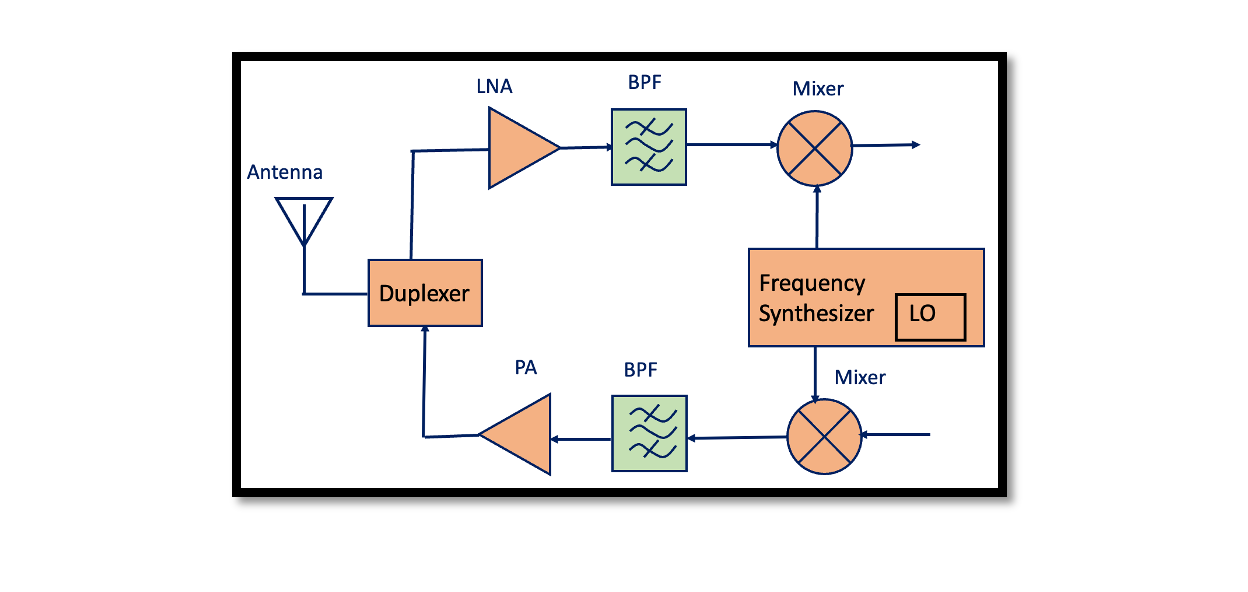
\includegraphics[scale=0.6]{img/tranceiver_structure.png}
	\end{center}
	\fonte{\citeonline{srakar_tranceiver_2023}.}
	\label{fig:tranceiver_structure}
\end{figure}


%%%%%%%%%%%%%%%%%%%%%%%%%%%%%%%%%%%%%%%%%%%%%%%%%%%%%%%%%%%%%%%%%%%%%%
\section{CMOS}
%%%%%%%%%%%%%%%%%%%%%%%%%%%%%%%%%%%%%%%%%%%%%%%%%%%%%%%%%%%%%%%%%%%%%%
CMOS (\textit{Complementary Metal-Oxide-Semiconductor}) é um processo de fabricação que utiliza silício para criar transistores de efeito de campo (MOSFETs) do tipo p e do tipo n, chamados de PMOS e NMOS, respectivamente. Amplamente utilizado na produção de chips de circuitos integrados, como microprocessadores, microcontroladores e chips de memória, o CMOS também é empregado em circuitos analógicos, como sensores de imagem e dispositivos de comunicação com e sem fio. Sua característica distintiva é o baixo consumo de energia, tornando-o especialmente adequado para dispositivos IoT.

Além disso, o CMOS oferece vantagens em relação a outras tecnologias, como operação em baixas tensões e uma evolução avançada que permite maior densidade de transistores por unidade de área . O tamanho dos transistores é determinado pelos valores de comprimento (L) e largura (W) Figura \ref{fig:nmos_structure}, permitindo um controle mais preciso da corrente que circula por eles \cite{designcmosrazavi2016}. Atualmente, circuitos integrados podem ser fabricados em escala de $3nm$ de acordo com dados da \textit{foundry} \cite{tsmc}.

\begin{figure}[h!]
	\caption{Estrutura de um NMOS}
	\begin{center}
		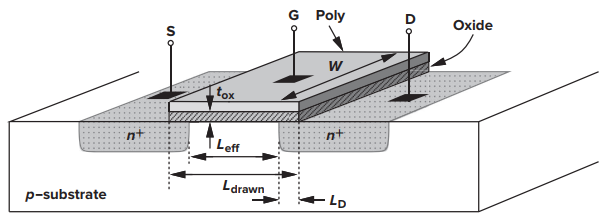
\includegraphics[scale=0.6]{img/nmos_structure.png}
	\end{center}
	\fonte{\citeonline{designcmosrazavi2016}.}
	\label{fig:nmos_structure}
\end{figure}

%%%%%%%%%%%%%%%%%%%%%%%%%%%%%%%%%%%%%%%%%%%%%%%%%%%%%%%%%%%%%%%%%%%%%%
\section{Bluetooth}
%%%%%%%%%%%%%%%%%%%%%%%%%%%%%%%%%%%%%%%%%%%%%%%%%%%%%%%%%%%%%%%%%%%%%%
O \textit{Bluetooth} é um padrão de tecnologia sem fio de curto alcance, amplamente utilizado para a troca de dados entre dispositivos fixos e móveis em distâncias curtas. 

Atualmente, milhões de pessoas em todo o mundo utilizam dispositivos \textit{Bluetooth} para transferir dados, como música, fotos e vídeos, no dia a dia. Além disso, o \textit{Bluetooth} tem sido cada vez mais empregado em dispositivos IoT, especialmente com a implementação do BLE (\textit{Bluetooth Low Energy}), que oferece maior alcance e menor consumo de energia em relação ao \textit{Bluetooth} padrão. Estima-se que em 2027 existirão cerca de 7,6 bilhões de dispositivos \textit{Bluetooth} ativos em todo o mundo \cite{BluetoothSite}.


Gerenciado pelo \textit{Bluetooth Special Interest Group} (SIG), o padrão opera no espectro de frequência $2,4GHz$. Na Tabela \ref{tab:bluetooth_specification} é apresentado algumas definições de comunicação \textit{Bluetooth} clássico e do BLE.

\begin{table}[h!]
	\caption{Definições de \textit{Bluetooth} clássico e BLE}
	
	\label{tab:bluetooth_specification}
	\resizebox{\columnwidth}{!}{%
		\begin{tabular}{lll}
			\hline
			& \textbf{\textit{Bluetooth} Low Energy (BLE)}      & \textbf{\textit{Bluetooth} Clássico}               \\ \hline
			\textbf{Banda de frequência} & 2.4 GHz Banda ISM  (2.402 – 2.480 GHz)    & 2.4 GHz Banda ISM  (2.402 – 2.480 GHz)    \\ \hline
			\textbf{Canais}              & 40 canais com 2 MHz de espaçamento        & 79 canais com 1 MHz de espaçamento       \\ \hline
			\textbf{Modulação}           & GFSK                                     & GFSK, $\pi$/4 DQPSK, 8DPSK                   \\ \hline
			\textbf{Uso do Canal}        & \textit{Frequency-Hopping Spread Spectrum} (FHSS) & \textit{Frequency-Hopping Spread Spectrum} (FHSS) \\ \hline
			\textbf{Data Rate (DR)}      & Até 2 Mb/s                                & Até 3 Mb/s                                \\ \hline
			\textbf{Sensibilidade (RX)}  & -82dBm com DR=120 kb/s                    & -70 dBm                                  \\ \hline
			\textbf{Topologia de comunicação} & \begin{tabular}[c]{@{}l@{}}Ponto a ponto\\ \textit{Broadcast}\\ \textit{Mesh}\end{tabular} & Ponto a ponto  \\ \hline
		\end{tabular}%		
	}
	\fonte{Adaptado de \citeonline{BluetoothSite}.}
\end{table}


%%%%%%%%%%%%%%%%%%%%%%%%%%%%%%%%%%%%%%%%%%%%%%%%%%%%%%%%%%%%%%%%%%%%%%
\section{Sintetizador de frequência}
%%%%%%%%%%%%%%%%%%%%%%%%%%%%%%%%%%%%%%%%%%%%%%%%%%%%%%%%%%%%%%%%%%%%%%
Em sistemas de comunicação sem fio a presença de um circuito sintetizador de frequência é essencial. O circuito sintetizador de frequência é responsável por gerar a frequência central de um canal em um sistema de comunicação de Rádio Frequência (RF). Cada canal possui uma faixa de frequência especifica de operação, desta forma o circuito do Sintetizador deve ser capaz de permitir ajustes de frequência pequenos.

O circuito Sintetizador de frequência gera as frequências necessária como um múltiplo de uma referência do Oscilador de Cristal Controlado por Temperatura (TXCO, do inglês \textit{Temperature-Controlled Crystal Oscillator}). O TXCO papel fundamental na performance do sintetizador, é responsavél por fornece uma frequência estável e precisa e com baixo valor de ruido de fase. De acordo com \cite{lascari2000accurate} negligenciar seus efeitos em um sintetizador pode acarretar em resultados inesperados após a concepção do circuito.

O processo de síntese de frequência ocorre através de técnicas de geração e mistura de sinais. Primeiramente, a referência de TXCO fornece uma frequência estável e precisa. Em seguida, o sintetizador de frequência utiliza circuitos internos, como divisores de frequência e circuitos de fase, para manipular e multiplicar a frequência da referência, produzindo assim a frequência desejada.


%%%%%%%%%%%%%%%%%%%%%%%%%%%%%%%%%%%%%%%%%%%%%%%%%%%%%%%%%%%%%%%%%%%%%%
\section{PLL}
%%%%%%%%%%%%%%%%%%%%%%%%%%%%%%%%%%%%%%%%%%%%%%%%%%%%%%%%%%%%%%%%%%%%%%
PLL (\textit{Phase-Locked-Lopp}) é um circuito Sintetizador de frequência comumente utilizado. PLL é composto por diversos blocos, alguns deles são: osciladores controlados por tensão VCO (\textit{Voltage-Controlled Oscillator}), divisores programáveis, comparadores de fase DFF (Detectores de Fase e Frequência), bombas de carga CP (\textit{Charge Pump}) e Filtros Passa Baixas LPF (\textit{Low Pass Filters}). 

Os blocos que compõem um PLL são apresentados na Figura \ref{fig:pll_blocks}.
A utilização de uma realimentação negativa no circuito permite um controle tanto de frequência como de fase para a saída.

\begin{figure}[h!]
	\caption{Diagrama de blocos de um PLL.}
	\begin{center}
		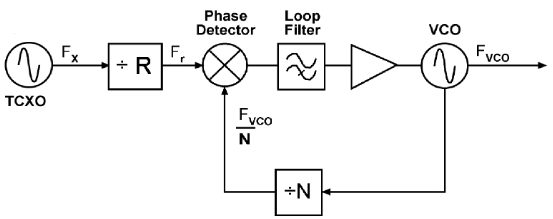
\includegraphics[scale=0.6]{img/pll_blocos.png}
	\end{center}
	\fonte{\citeonline{barrett_1999_fractionalintegern}.}
	\label{fig:pll_blocks}
\end{figure}

O PLL utiliza o VCO como elemento central. O sinal de saída do VCO, dividido por um fator N, é comparado com a frequência de referência do TXCO, dividida por R, pelo  \textit{Phase-Detector}. Após a comparação, o sinal resultante passa pelo \textit{Loop filter}, responsável por eliminar ruídos e interferências. A saída do \textit{Loop filter} é uma tensão que controla a tensão aplicada ao VCO, permitindo ajustar e manter a frequência de saída em sincronia com a frequência de referência \cite{barrett_1999_fractionalintegern}.

Em condições normais, um PLL fornece uma frequência com extrema precisão, no entanto, o tempo de aquisição pode ser longo devido ao processo do detector de fase e frequência em avaliar e gerar sinais com base nas diferenças em relação à referência. Esse tempo de aquisição é especialmente crucial em aplicações de comunicações sem fio que envolvem técnicas como salto de canal (\textit{frequency hopping}), como é o caso do protocolo \textit{Bluetooth}. Nessas situações, a capacidade do PLL de se sincronizar rapidamente com frequências variáveis é essencial para garantir uma transição suave entre os canais e evitar perdas de dados ou conexão.
%%%%%%%%%%%%%%%%%%%%%%%%%%%%%%%%%%%%%%%%%%%%%%%%%%%%%%%%%%%%%%%%%%%%%%
\subsection{Integer-N PLL}
%%%%%%%%%%%%%%%%%%%%%%%%%%%%%%%%%%%%%%%%%%%%%%%%%%%%%%%%%%%%%%%%%%%%%%

PLLs convencionais também conhecidos como \textit{Integer-N PLL} são capazes de gerar apenas frequências de valores N vezes a frequência do TXCO, onde N é um valor inteiro, desta forma a resolução de frequência é definida pela frequência de referência utilizada. 

A frequência de saída é definida como:

\begin{equation}
	F_{VCO} = N \cdot F_{ref}
	\label{eq:fvco_integer_PLL}
\end{equation}



%%%%%%%%%%%%%%%%%%%%%%%%%%%%%%%%%%%%%%%%%%%%%%%%%%%%%%%%%%%%%%%%%%%%%%
\subsection{Fractional-N PLL}
%%%%%%%%%%%%%%%%%%%%%%%%%%%%%%%%%%%%%%%%%%%%%%%%%%%%%%%%%%%%%%%%%%%%%%
Em um \textit{fractional-N} PLL a frequência de saída pode ser ajustada como uma fração da frequência de referência. Esse ajuste fracional é necessário em sistemas de comunicação para o ajuste correto da frequência central de canal utilizado. 

\textit{Fractional-N} PLL utiliza uma topologia similar ao do \textit{Integer-N} PLL, com adição de um acumulador, uma maquina de alterna o divisor entre (N e N+1) durante um estado bloqueado. Esta variação faz com que a média torne-se um valor fracional entre N e N+1, proporcionando um ajuste de frequência também fracional. 

A frequência de saída é definida como:

\begin{equation}
	F_{VCO} = (N + F) \cdot F_{ref}
	\label{eq:fvco_fractional_PLL}
\end{equation}
Onde, $F$ é $0$ ou $1$. 

%%%%%%%%%%%%%%%%%%%%%%%%%%%%%%%%%%%%%%%%%%%%%%%%%%%%%%%%%%%%%%%%%%%%%%
\section{ADPLL}
%%%%%%%%%%%%%%%%%%%%%%%%%%%%%%%%%%%%%%%%%%%%%%%%%%%%%%%%%%%%%%%%%%%%%%

O ADPLL (\textit{All Digital Phase-Locked-Loop}) é um sintetizador de frequência que se diferencia dos PLLs convencionais por ser um circuito puramente digital. Enquanto um PLL tradicional requer componentes analógicos, como capacitores, resistores e indutores, o ADPLL aproveita os benefícios da miniaturização da tecnologia CMOS, permitindo maiores velocidades e frequências, além de reduzir significativamente a área ocupada no chip.

Para \cite{staszewski2006all} a tecnologia nanométrica do CMOS traz um novo paradigma, a resolução do domínio do tempo de uma transição de borda de sinal digital é superior à resolução de tensão de sinais analógicos. Desta forma o ADPLL pode ser analisado apenas pelas transições dos sinais digitais.

A natureza digital do ADPLL oferece vantagens adicionais, como a parametrização do \textit{Loop-Filter} para ajuste de frequência conforme necessário. Além disso, não são necessários circuitos auxiliares para conversão entre sinais digitais e analógicos, o que representa uma economia de recursos e simplificação do projeto.

A Figura \ref{fig:adpll_block_diagram} mostra o diagrama de blocos de um ADPLL no domínio do tempo discreto, ou seja considerando as transições dos sinais de (FREF) e saída do circuito (DCO). O ADPLL é composto de 4 blocos principais,  \textit{Digital Controlled Oscillator} (DCO), \textit{Time to Digital Converter} (TDC), \textit{Phase Detector} (PD) e o \textit{ digital Loop Filter} (LF). Nas subseções seguintes serão apresentados com mais detalhes cada um dos sub-blocos. 

\begin{figure}[h!]
	\caption{Diagrama de blocos de um ADPLL.}
	\begin{center}
		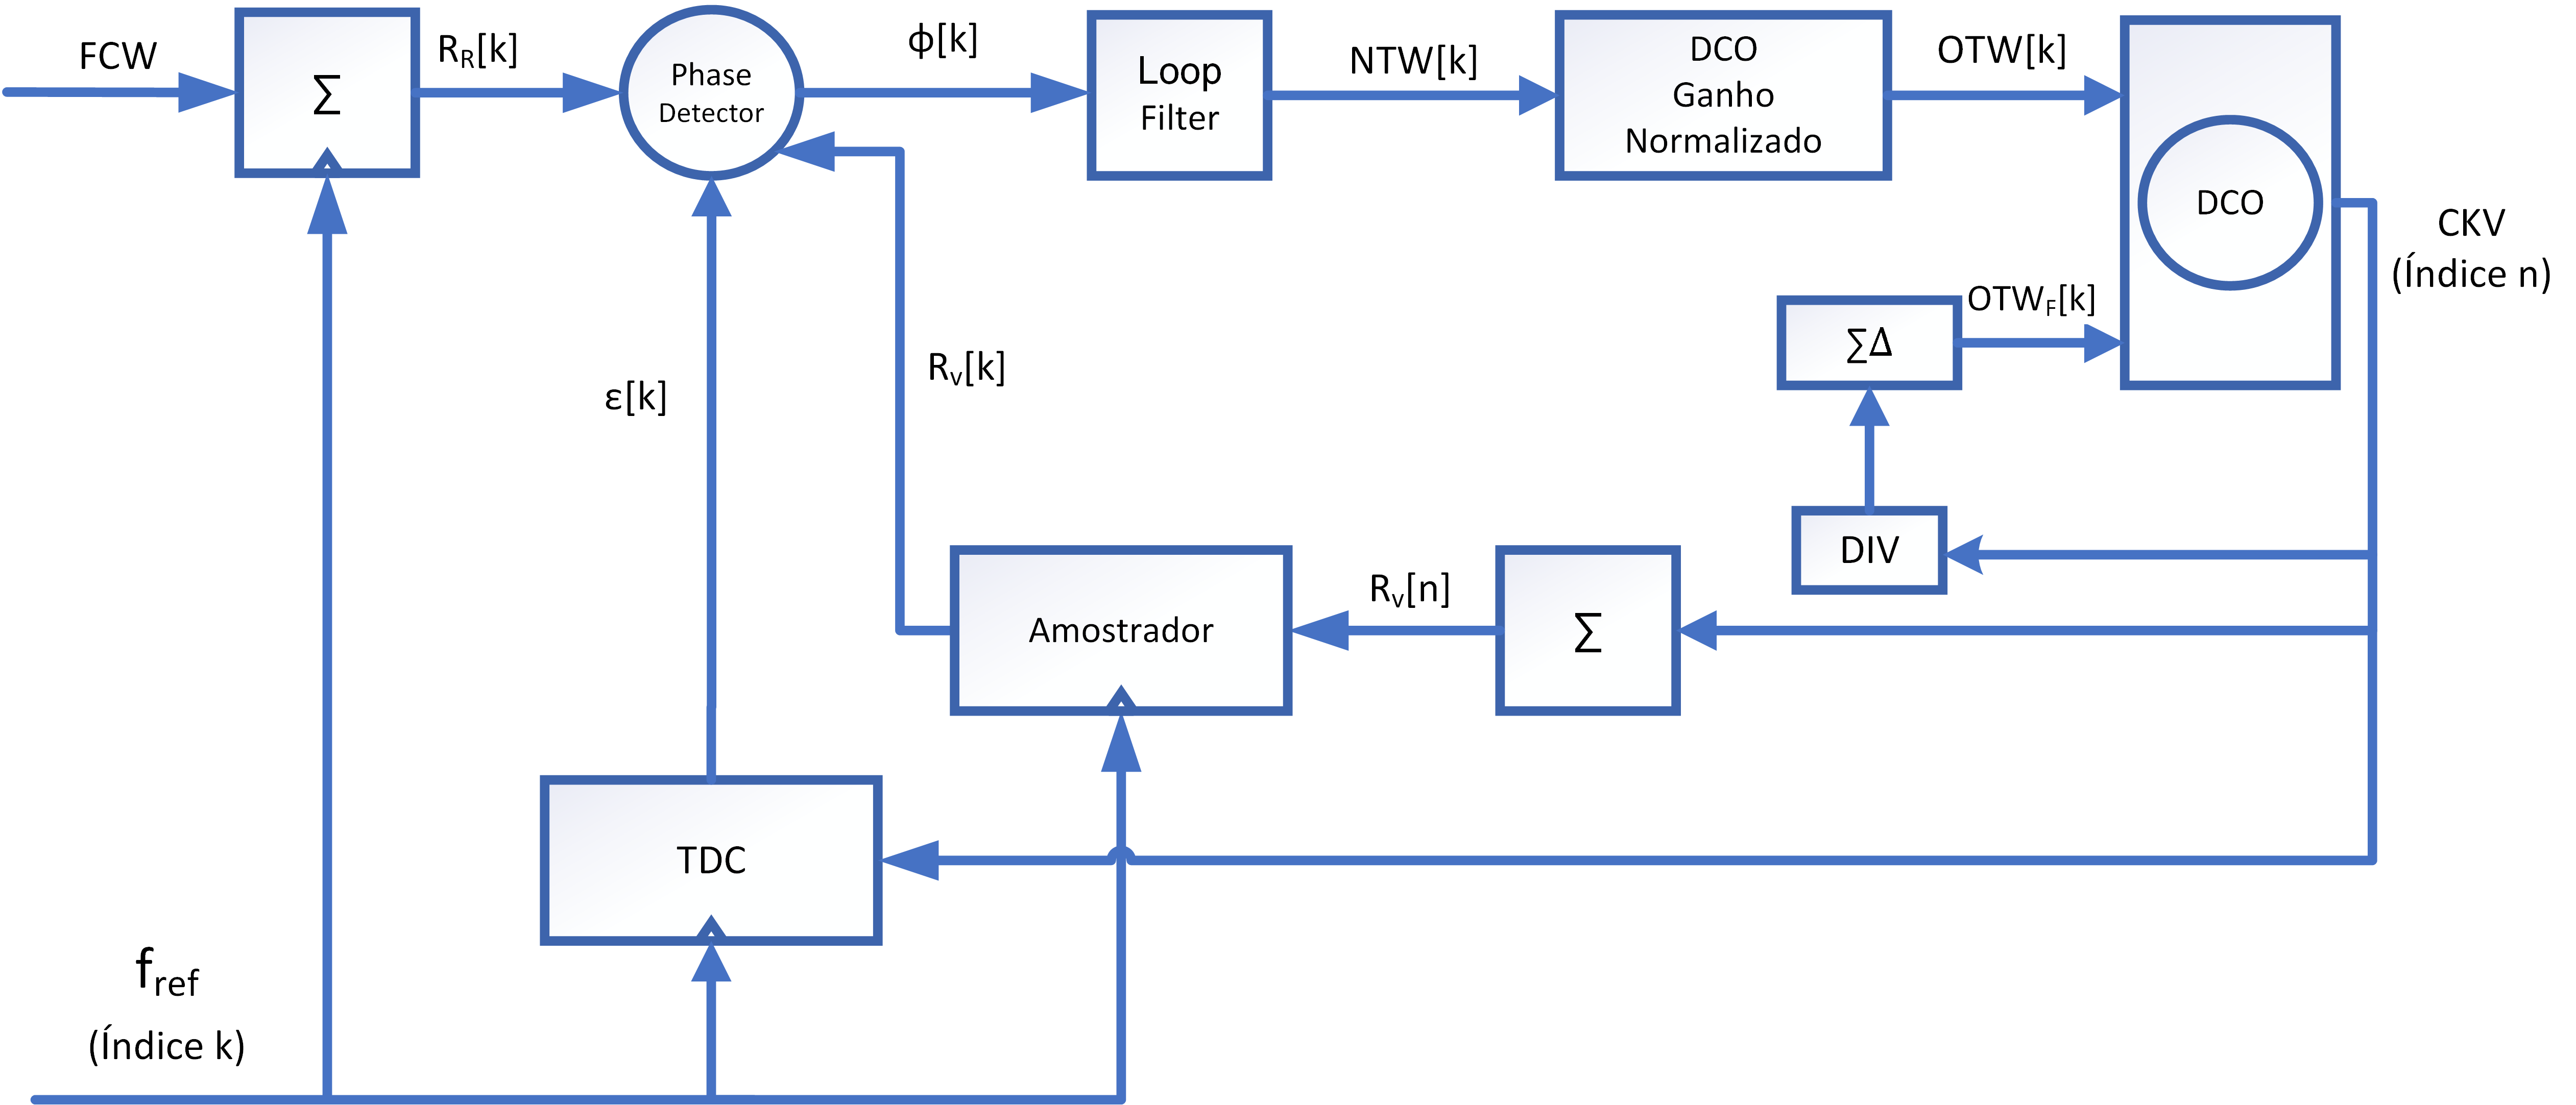
\includegraphics[scale=1]{img/blocos_ADPLL.png}
	\end{center}
%	\fonte{\citeonline{staszewski2006all}}
\fonte{Adaptado de \citeonline{andersson2010modeling}.}
	\label{fig:adpll_block_diagram}
\end{figure}

O circuito do DCO é responsável por gerar o sinal de saída do sintetizador. Ele consiste em um indutor fixo e um conjunto de capacitores programáveis que formam um circuito ressonante LC. A frequência de saída é definida pelo FCW (\textit{Frequency Command Word}), pode ser um valor fracionado ou inteiro da frequência de referência, conforme expresso na Equação \ref{eq:fvco_adpll}.

\begin{equation}
	F_{VCO} = FCW \cdot F_{ref}
	\label{eq:fvco_adpll}
\end{equation}

Por outro lado, o TDC realiza a medição da diferença de tempo entre as bordas de \textit{clock} do sinal do DCO e uma borda de referência, , acumulando esse valor a cada transição do \textit{clock}, da mesma forma que FCW. O detector de fase compara as diferenças entre os acumuladores, que é então utilizado pelo \textit{Loop Filter} para controlar os capacitores do DCO. Essa ação de controle resulta no ajuste da frequência do sinal de saída, permitindo aumentá-la ou reduzi-la conforme necessário.

%%%%%%%%%%%%%%%%%%%%%%%%%%%%%%%%%%%%%%%%%%%%%%%%%%%%%%%%%%%%%%%%%%%%%%
\subsection{DCO}
%%%%%%%%%%%%%%%%%%%%%%%%%%%%%%%%%%%%%%%%%%%%%%%%%%%%%%%%%%%%%%%%%%%%%%

O DCO é o elemento principal do ADPLL, converte o \textit{Oscilator Tunning Word}, ($OTW$), em um sinal periódico onde a frequência $f$ é definida em função de sua entrada.
\begin{equation}
	f = f(OTW)
	\label{eq:f_OTW}
\end{equation}

O DCO é formado por um circuito tanque LC, um indutor fixo e capacitores programáveis, em ressonância a frequência é definida de acordo com a equação \ref{eq:f_LC} onde $C_{tot}$ é a soma de todas capacitâncias.

\begin{equation}
	f_{out} = \frac{1}{2 \pi \sqrt{L \cdot C_{tot}}}
	\label{eq:f_LC}
\end{equation}

Transistores em modo varactor são utilizado como capacitores programáveis, pois possuem um ajuste muito pequeno de frequência em relação a varactores de diodo. Quanto menor o valor da capacitância menor é o  passo de frequência de ajuste do DCO, permitindo um ajuste mais fino e melhor performance. 

Transistores do tipo PMOS são comumente utilizados como varactores devido a suas propriedades de isolação do poço. Com os terminais dreno, fonte e corpo (D=S=B) interligados permite que a capacitância seja controlada pelo nível de tensão $VG$ conforme a região de operação do transistor, limitada pela capacitância do óxido $(C_{OX})$. A Figura \ref{fig:curva_COX_vbg} mostra a curva de capacitância em relação a tensão aplicada ao terminal gate.

\begin{figure}[h!]
	\caption{Curva de resposta do varactor D=S=B em relação a $VG$ }
	\begin{center}
		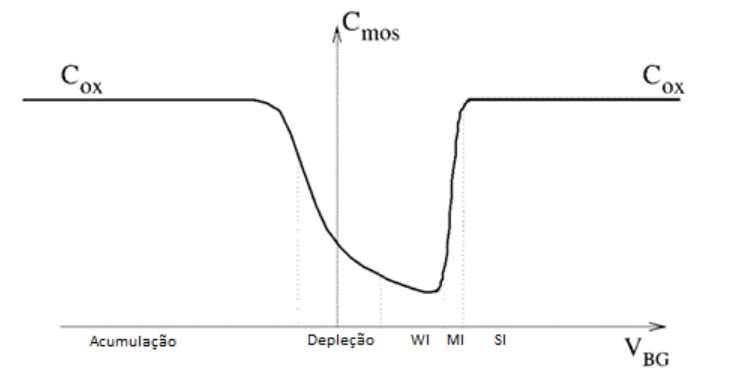
\includegraphics[scale=0.6]{img/curva_COX_vbg.png}
	\end{center}
	\fonte{\citeonline{lucasvco2022}.}
	\label{fig:curva_COX_vbg}
\end{figure}

O DCO deve ser capaz de gerar um range de frequências com ajuste fino para atender às necessidades de modulação do transceptor. Por exemplo, para o \textit{Bluetooth}, que possui um range de frequências entre $2.402GHz$ e $2.480GHz$, usar apenas 8 bits, um conjunto de 256 capacitores programáveis, resultaria em um passo de frequência muito grosso de aproximadamente $304,67kHz$, o que não é viável para aplicações sem fio e tipos de modulações utilizadas.

Para superar essa limitação, a solução adotada é dividir o banco de capacitores em três partes: modo de Processo-Tensão-Temperatura (PVT), modo de aquisição (ACQ) e modo de caminhada (TRK). Esses modos permitem ajustar o DCO de maneira mais precisa. De acordo com \cite{staszewski2006all}, uma boa relação entre tamanho físico e menor passo de frequência é alcançada atribuindo 8 bits para o modo PVT, 8 bits para o modo ACQ e 6 bits para o modo TRK.

Na Figura \ref{fig:bank_modos} é apresentado o fluxo de operação dos modos do DCO. Cada modo possui um range de frequência de operação, e a mudança de uma unidade no $OTW$ define o menor passo de frequência,  $\Delta f$ possível em cada modo . Este passo pode ser calculado para cada modo conforme a equação \ref{eq:step_freq_mode}, considerando o range de frequência e o numero de bits em cada um. 
\begin{equation}
	\Delta f_{LSB_{mode}} = \frac{F.R_{mode}}{2^{b_{mode}}}
	\label{eq:step_freq_mode}
\end{equation}

\begin{figure}[h!]
	\caption{Fluxo de operação dos modos do DCO }
	\begin{center}
		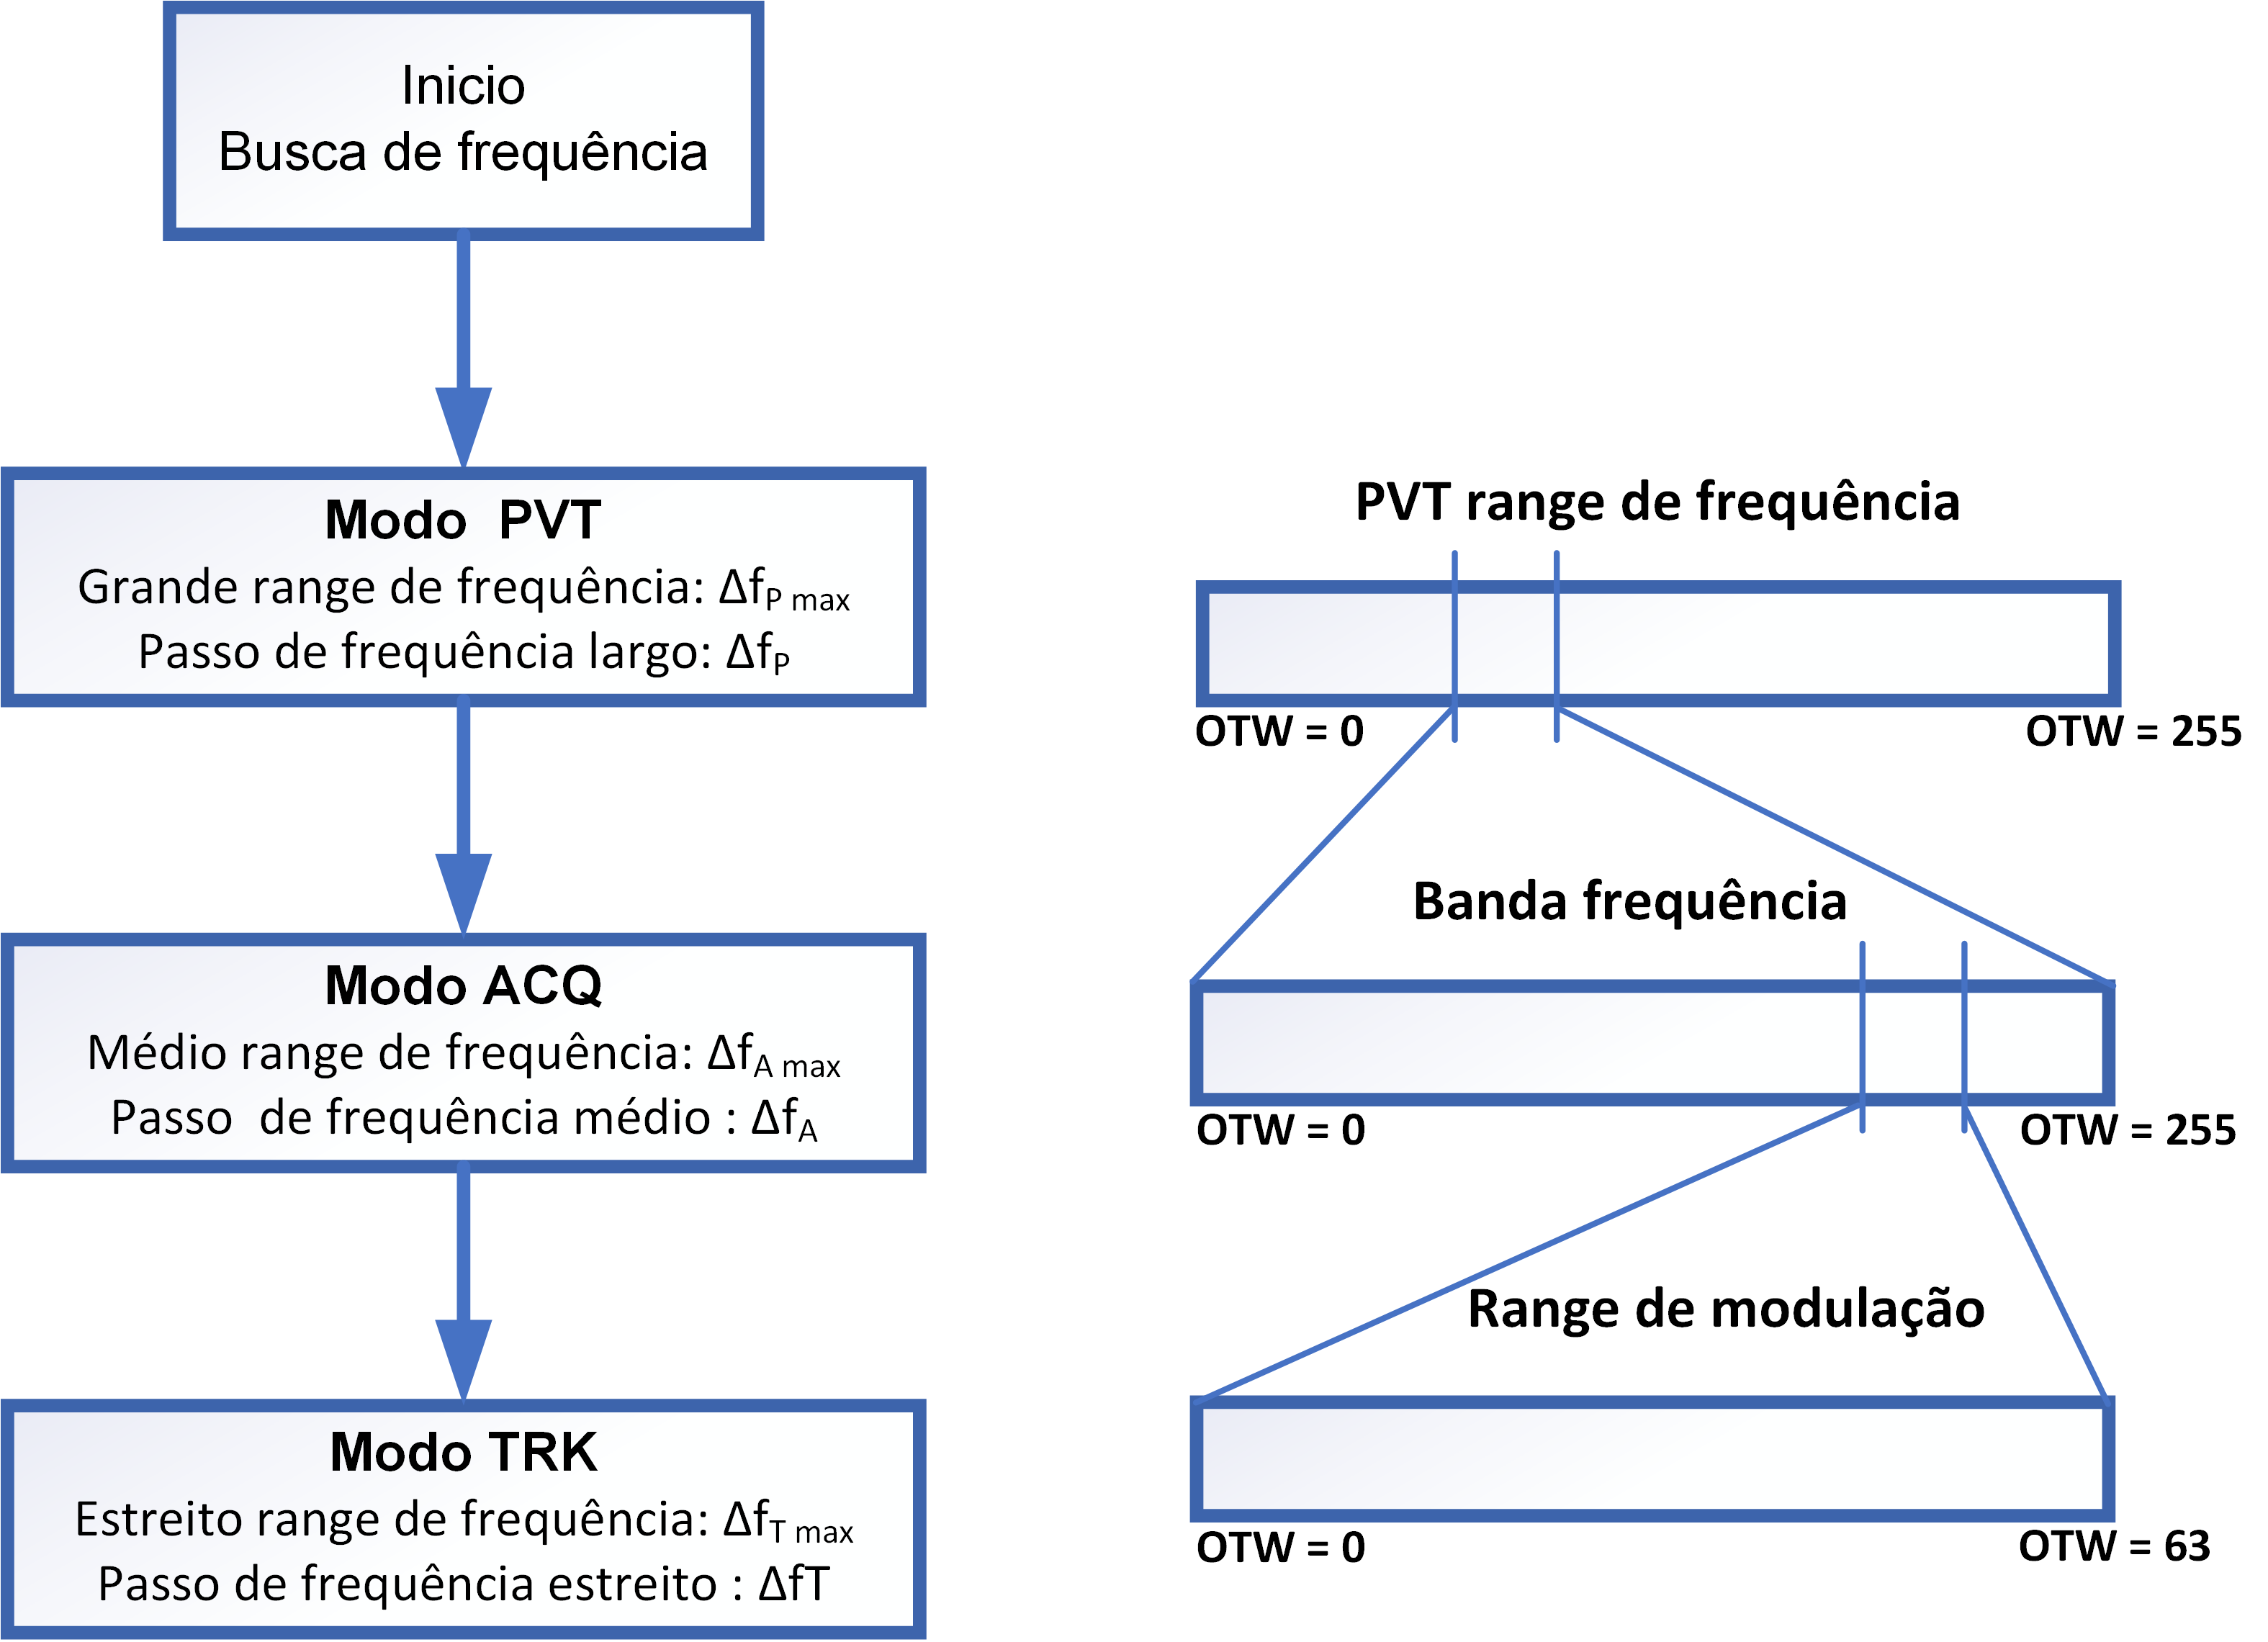
\includegraphics[scale=0.6]{img/bank_modos.png}
	\end{center}
	\fonte{Adaptado de \citeonline{staszewski2006all}.}
	\label{fig:bank_modos}
\end{figure}

Ao iniciar o DCO, todos os modos são iniciados no centro do range de ajuste, com um valor de $OTW=127$ para PVT e ACQ e $OTW=33$ para TRK. Configurar $OTW$ como $0$ corresponde à menor frequência possível, enquanto $255$ representa a frequência mais alta. O modo PVT é o primeiro a ser ajustado fazendo a compensação de variações de processo, temperatura e tensão, centralizando a frequência do oscilador de forma mais grosseira, apresentando variações entre $1$ a $2MHz$.

No segundo modo, ACQ, a frequência é ajustada para dentro da banda de interesse com um passo de frequência médio $\Delta f_A$, fornecendo uma resolução de $\pm 500kHz$ ao variar $OTW$ entre 0 e 255.

Por fim, o modo TRK possui a melhor resolução de ajuste, permitindo ajustar com precisão a frequência de saída do oscilador necessária para a modulação do sinal. Para permitir ajustes muito finos, como $\pm 1kHz$, $OTW$ pode ser um valor fracionário nesse modo. Para isso, é utilizada uma topologia semelhante à do \textit{Fractional-N PLL}, permitindo uma melhor resolução com a implementação de um modulador Sigma-Delta (SDM). Os SDMs são amplamente utilizados em conversores ADs (analógico para digital) por meio de um modulador com sobre-amostragem, seguido por um filtro digital/decimador, que juntos produzem um sinal de alta resolução \cite{sdmtexas}. Essa técnica de modulação é empregada para alcançar um ajuste preciso e refinado da frequência do DCO, garantindo a adequada modulação do sinal dentro do canal designado.


A Figura \ref{fig:lc_bank_capacitor} apresenta o tanque LC de um DCO projetado para aplicação \textit{Bluetooth}, com a implementação dos três bancos de capacitores. Nos bancos PVT e ACQ cada capacitor representado por um bit possui um mesmo valor conforme o banco que ele pertence, a soma deles em conjunto com o capacitor $C_0$ definirá a frequência. 

\begin{figure}[h!]
	\caption{Tanque LC com banco de capacitores para aplicação \textit{Bluetooth} }
	\begin{center}
		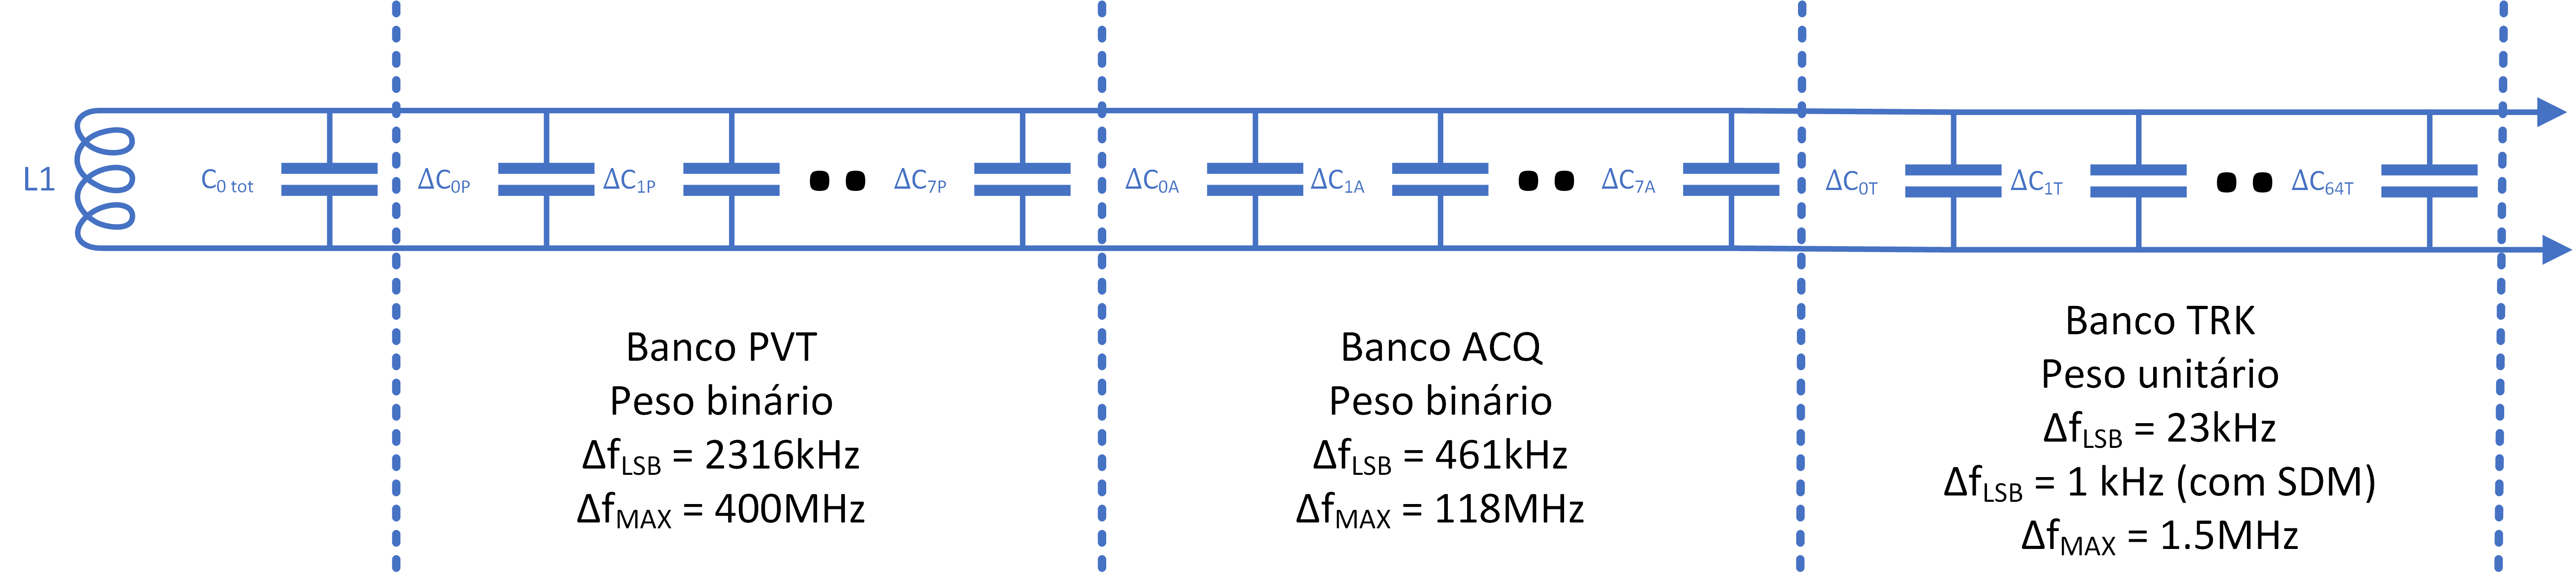
\includegraphics[scale=0.8]{img/lc_bank_capacitor.png}
	\end{center}
	\fonte{Adaptado de \citeonline{staszewski2006all}.}
	\label{fig:lc_bank_capacitor}
\end{figure}


Nos bancos de capacitores PVT e ACQ o valor individual de cada capacitor é definido pela equação \ref{eq:c_delta}, na qual leva em consideração a frequência minima e máxima de operação de cada banco. O valor de $C_0$ é igual ao valor de $C_{min}$ do banco PVT, ou seja é a máxima frequência do oscilador.
\begin{equation}
	C_{max} = \frac{1}{L} \big( \frac{1}{2 \pi f_{min}} \big)^2
	\label{eq:cmax}
\end{equation}

\begin{equation}
	C_{min} = \frac{1}{L} \big( \frac{1}{2 \pi f_{max}} \big)^2
	\label{eq:cmin}
\end{equation}

\begin{equation}
	\Delta C^{banco} = \frac{	C_{max} - C_{min}}{2}
	\label{eq:c_delta}
\end{equation}

Após o ajuste do banco PVT a capacitância total é obtida pela equação \ref{eq:c_A_total}, considerando o número de capacitores acionados considerando o valor de cada um e também a metade dos capacitores dos bancos ACQ e TRK acionados.

\begin{equation}
	C^P = C_0 + C^A_{half} + C^T_{half} + \sum_{k=0}^{7} \bar{d}_k \cdot 2^k * 	\Delta C^P
	\label{eq:c_P_total}
\end{equation}

Da mesma forma após o ajuste do banco ACQ a capacitância total é obtida pela equação \ref{eq:c_A_total} considerando o valor do banco PVT já ajustado.
\begin{equation}
	C^A = C_P - C^A_{half} + C^T_{half} + \sum_{k=0}^{7} \bar{d}_k \cdot 2^k * 	\Delta C^A
	\label{eq:c_A_total}
\end{equation}


No modo TRK os capacitores são rearranjados de forma diferente. Utilizando peso binário quando $OTW$ mudar de 31 para 32 fara com que 6 capacitores sejam alterados, causando bordas de ruído no sinal de saída, o que não é desejável visto que neste modo é importante manter a estabilidade para garantir a comunicação.   Desta forma no modo TRK cada capacitor possui valor unitário, ou seja a mudança de $OTW$ fara com que apenas um capacitor seja alterado, evitando ruídos indesejados. O valor de cada capacitor é calculado conforme a equação \ref{eq:c_unit_TRK}, considerando o range de frequência necessário e o número de bits utilizado no modo. 

\begin{equation}
	C_\mu = \frac{	C_{max} - C_{min}}{2^{bTRK}}
	\label{eq:c_unit_TRK}
\end{equation}

Por fim a capacitância total do tanque LC pode ser obtida pela equação \ref{eq:c_T_total} ao final do ajuste do banco TRK, sendo a soma das capacitâncias dos bancos anteriores com o atual. Desta forma $C^T = C_{tot}$ e pode ser utilizada a equação \ref{eq:f_LC} para estimar a frequência de saída do oscilador.
\begin{equation}
	C^T = C_A -  C^T_{half} + (2^{bTRK} - OTW) \cdot 	C_\mu
	\label{eq:c_T_total}
\end{equation}


%%%%%%%%%%%%%%%%%%%%%%%%%%%%%%%%%%%%%%%%%%%%%%%%%%%%%%%%%%%%%%%%%%%%%
\subsubsection{Ganho Normalizado}
%%%%%%%%%%%%%%%%%%%%%%%%%%%%%%%%%%%%%%%%%%%%%%%%%%%%%%%%%%%%%%%%%%%%%%


A frequência de saída do DCO é definida em função da entrada ($OTW$), sendo $f_{out} = f(OTW)$. Essa função não é linear, mas pode ser aproximada a uma função linear considerando um pequeno range de operação. Neste caso $f(OTW)$ é um simples ganho $K_{DCO}$, podendo ser escrito como:

\begin{equation}
	f_{out} = f_0 + \Delta f_v = f_o + K_{DCO} \cdot OTW
	\label{eq:deltaf_ndco}
\end{equation}

Onde $\Delta f$ é um desvio da frequência central $f_0$. o ganho$K_{DCO}$ é definido como o desvio de frequência em resposta a mudança de 1 bit, LSB, em $OTW$. 

Cada um dos três modos de operação do DCO possui um range de frequência diferente, , o que resulta em diferentes valores de ganho.  O cálculo do ganho é efetuado pela equação \ref{eq:kdco_mode} considerando o range de frequência e o numero de bits utilizado em cada modo.




\begin{equation}
	K_{DCO_{mode}}= \frac{F \ cdot R_{mode}}{2^{b_{mode}}}
	\label{eq:kdco_mode}
\end{equation}

A Figura \ref{fig:ndco} mostra o bloco de um ganho normalizado, onde  NTW (\textit{Normalized Tunning Word}) é normalizado em OTW pela frequência de referência($f_{ref}$) dividida pelo ganho($	K_{DCO}$).

\begin{figure}[h!]
	\caption{Diagrama de blocos do ganho normalizado }
	\begin{center}
		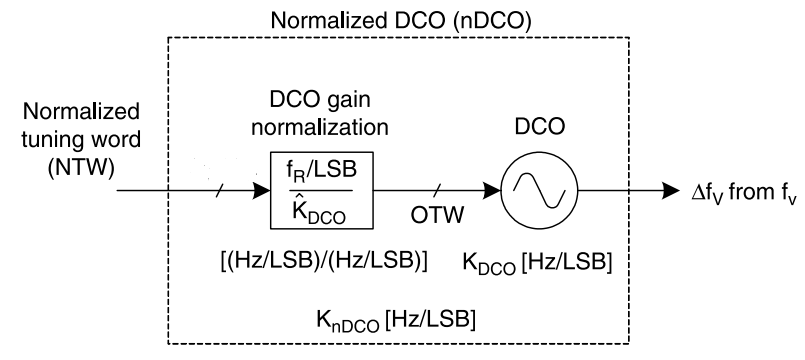
\includegraphics[scale=0.8]{img/ndco.png}
	\end{center}
	\fonte{ \citeonline{StaszewskinDCO}.}
	\label{fig:ndco}
\end{figure}

Devido ao fato do ganho sofrer por variações variações de processo e de fatores ambientais, não se pode definir com precisão seu valor.Para minimizar isto é utilizado uma estimativa de ganho conforme a equação \ref{eq:kdco_est}. Se  $K_{DCOest}$ for corretamente estimado, o ganho torna-se igual a $f_{ref}$, e as alterações em \textit{NTW} acarretam em alteração da frequência na mesma magnitude, multiplicada por $f_{ref}$.

\begin{equation}
	K_{nDCO}=  f_{ref}\frac{K_{DCO}}{K_{DCOest}}
	\label{eq:kdco_est}
\end{equation}


É fundamental obter um valor preciso para o ganho $K_{DCO}$ a fim de garantir a acurácia do sintetizador, especialmente no modo TRK, onde é necessária a maior precisão.

%%%%%%%%%%%%%%%%%%%%%%%%%%%%%%%%%%%%%%%%%%%%%%%%%%%%%%%%%%%%%%%%%%%%%%
%\subsection{Modulador Sigma Delta}
%%%%%%%%%%%%%%%%%%%%%%%%%%%%%%%%%%%%%%%%%%%%%%%%%%%%%%%%%%%%%%%%%%%%%%


%%%%%%%%%%%%%%%%%%%%%%%%%%%%%%%%%%%%%%%%%%%%%%%%%%%%%%%%%%%%%%%%%%%%%
\subsection{Phase detector}
%%%%%%%%%%%%%%%%%%%%%%%%%%%%%%%%%%%%%%%%%%%%%%%%%%%%%%%%%%%%%%%%%%%%%%
\textit{Phase detector } mede a diferença de fase entre o sinal de referência e a saída do sintetizador a cada borda de \textit{clock} da referência. A Figura \ref{fig:phase_detector_block} demonstra o diagrama de blocos do \textit{Phase detector}.

\begin{figure}[h!]
	\caption{Phase detector}
	\begin{center}
		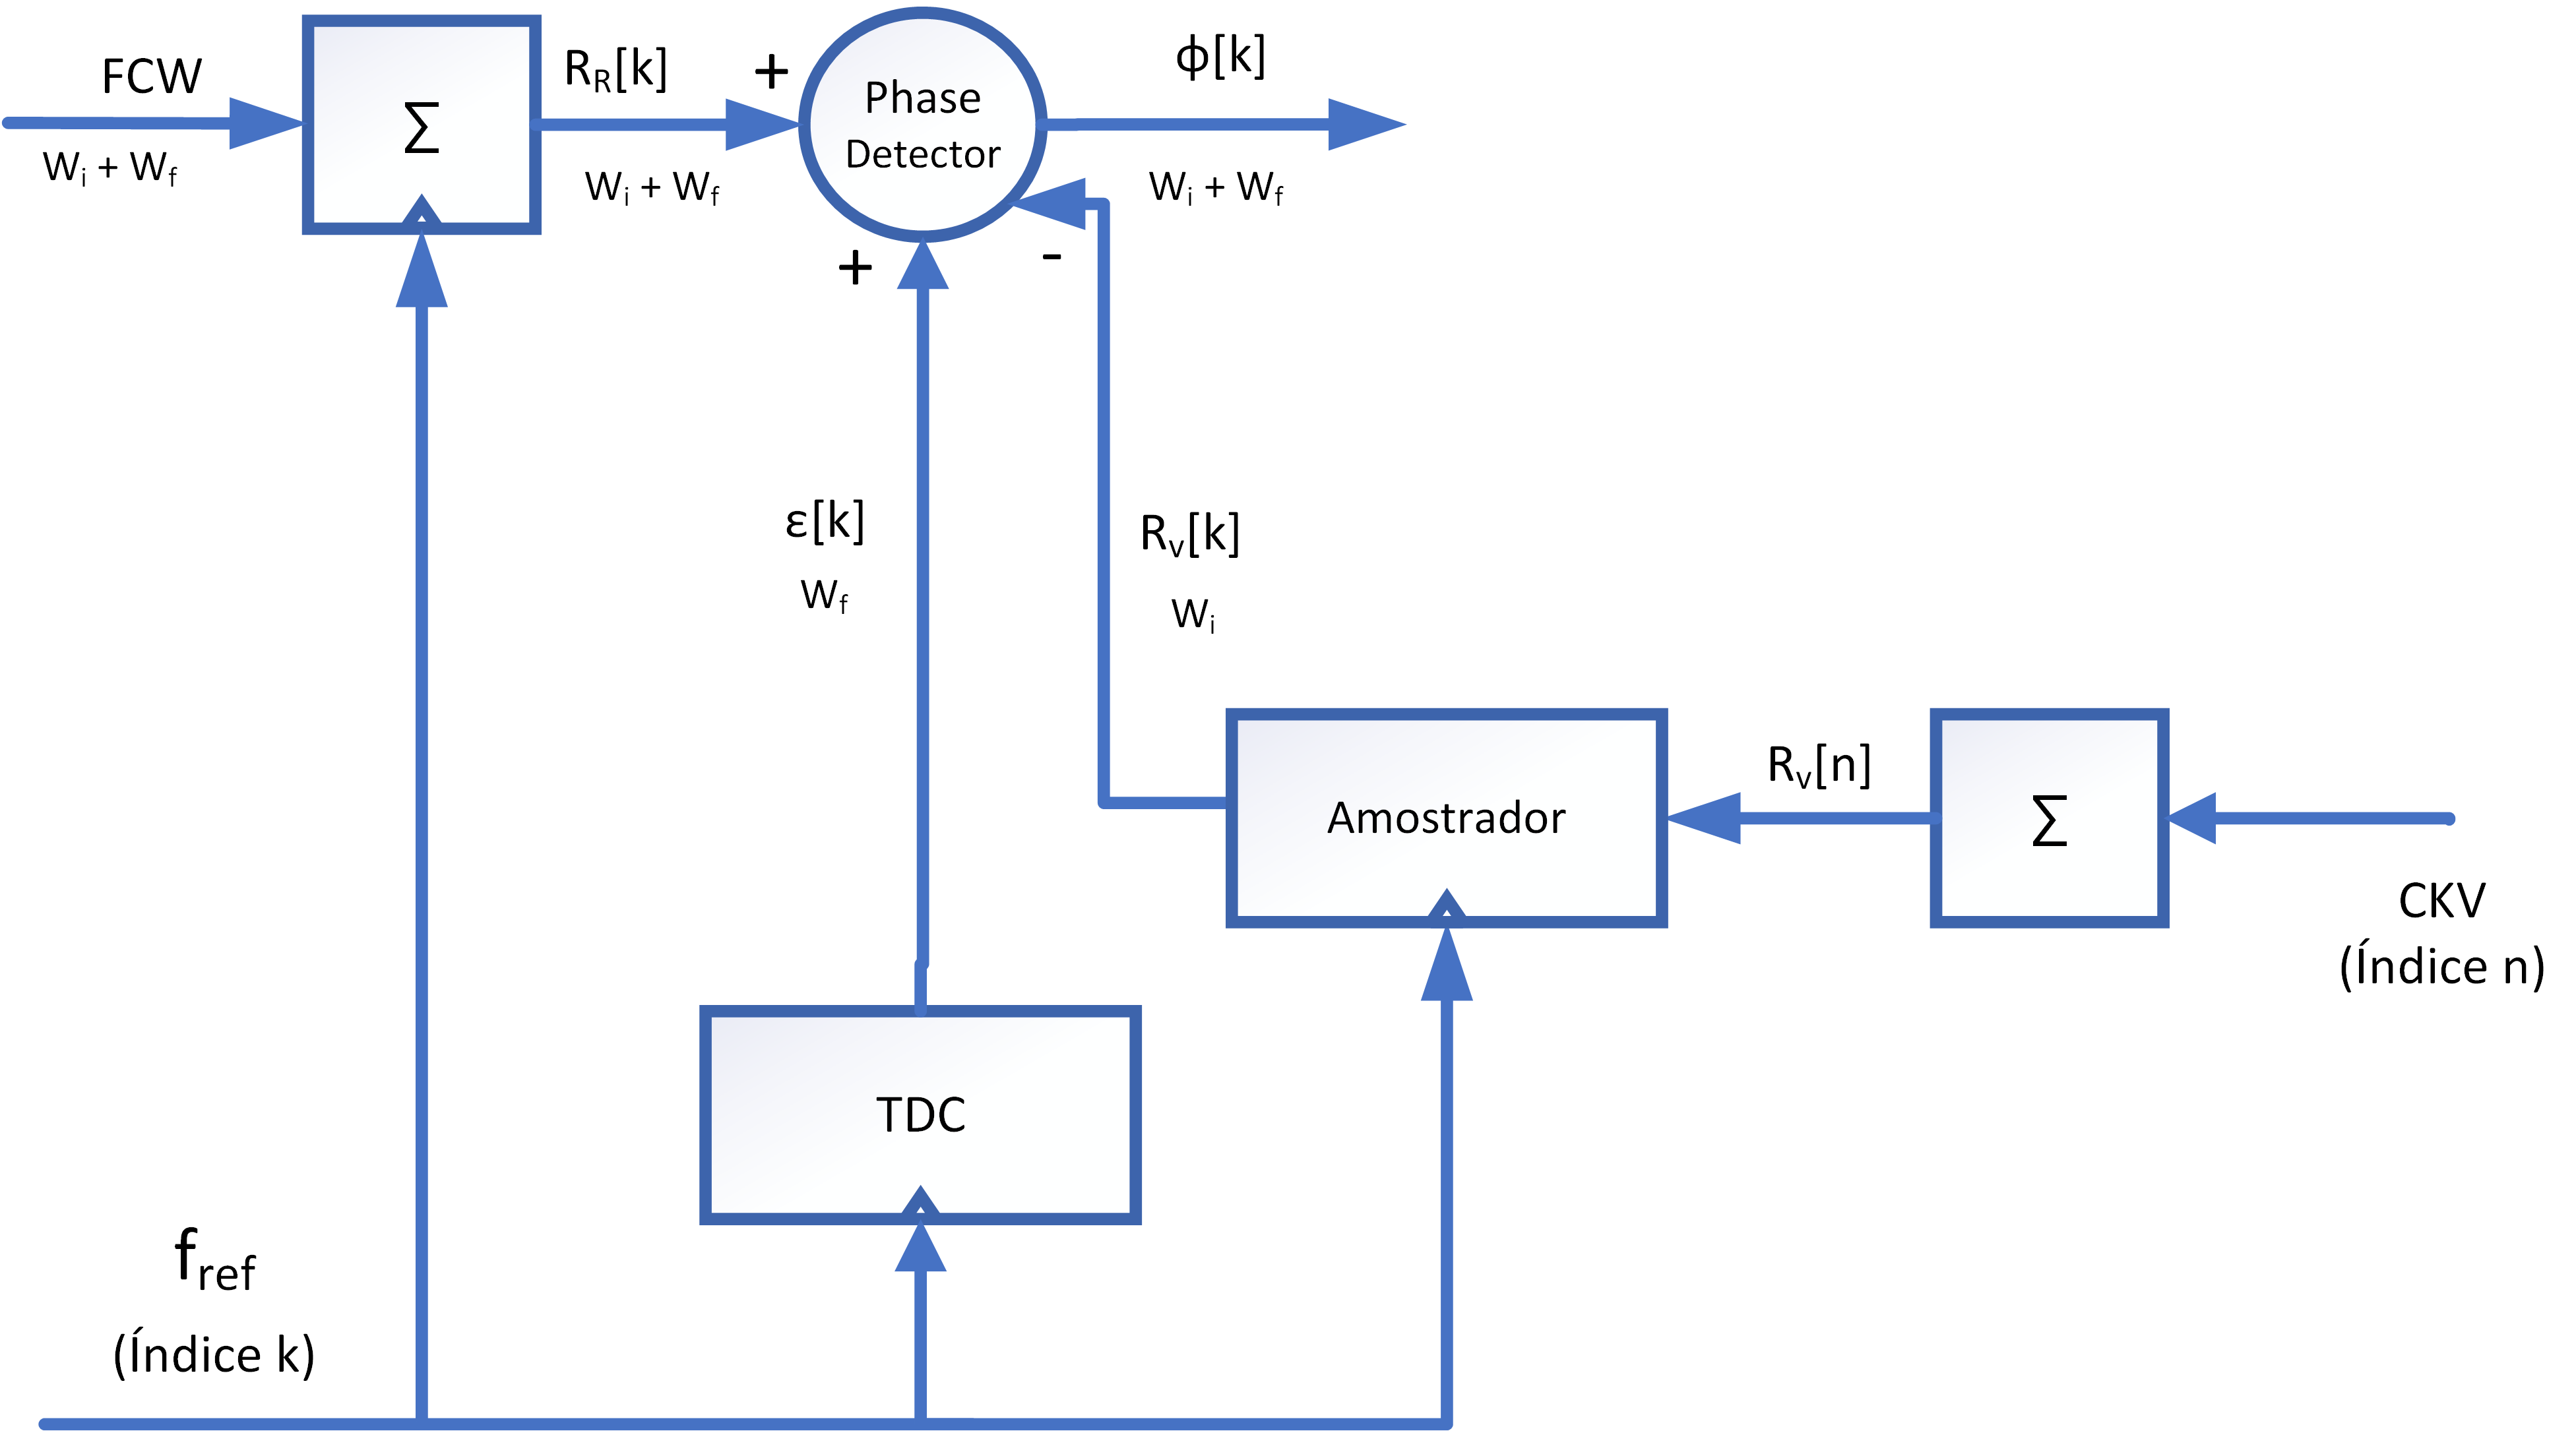
\includegraphics[scale=0.8]{img/phase_detector_block.png}
	\end{center}
	\fonte{Elaborado pelo autor(2023).}
	\label{fig:phase_detector_block}
\end{figure}

O valor de FCW que define a frequência de saída do circuito de acordo com a equação \ref{eq:fvco_adpll}, possui uma parte inteira $W_i$ e uma parte fracional $W_f$. 
 A cada borda de \textit{clock} de $f_{ref}$, índice $k$, o valor de FCW é acumulado $R_R[k] = R_R[k-1] + FCW$, representando a fase de referência. A fase variável $R_V[k]$ acumulada o número de bordas CKV, e o erro fracional é obtido pelo TDC que será apresentado na seção seguinte.

A saída do \textit{Phase detector } é o erro de fase $\phi$ entre os sinais calculada conforme a equação \ref{eq:phase_detector}.Quando o ADPLL converge para a fase e frequência desejada a saída $\phi$ será uma constante.

 \begin{equation}
	\phi [k]= R_R[k] - ( R_V[k] - \epsilon[k]) =  (R_{R_{Int}}[k] - R_V[k]) + ( R_{R_{Frac}}[k] - \epsilon[k])
	\label{eq:phase_detector}
\end{equation}
%%%%%%%%%%%%%%%%%%%%%%%%%%%%%%%%%%%%%%%%%%%%%%%%%%%%%%%%%%%%%%%%%%%%%
\subsection{Loop Filter}
%%%%%%%%%%%%%%%%%%%%%%%%%%%%%%%%%%%%%%%%%%%%%%%%%%%%%%%%%%%%%%%%%%%%%%
\label{sec:loop_filter}

O \textit{Loop Filter} é um sistema de controle do tipo PI (proporcional e integral) responsável por regular o NTW (\textit{Normalized Tunning Word}). Ele recebe como entrada a diferença de fase entre a referência e a saída do DCO, e sua saída é aplicada ao bloco do ganho normalizado, que controla o DCO. O \textit{Loop Filter} é responsável pela estabilidade e precisão do ADPLL, garantindo que a frequência e fase de saída do DCO seja mantida próxima à frequência de referência.

Na Figura \ref{fig:loop_filter_PI}, é apresentada a estrutura básica de um sistema de controle PI, enquanto a Figura \ref{fig:loop_filter_typeII} ilustra sua análise no domínio Z. O parâmetro $K_p$ representa o ganho proporcional e determina a velocidade do sistema, ou seja, quão rapidamente ocorre a mudança na saída dada uma variação na entrada. Já $K_i$ atua como um integrador, ajudando a eliminar erros estacionários, garantindo a estabilidade do sistema e reduzindo o impacto de perturbações externas.

\begin{figure}[h!]
	\caption{\textit{Loop Filter} }
	\begin{center}
		\subfloat[Controlador PI convencional]{	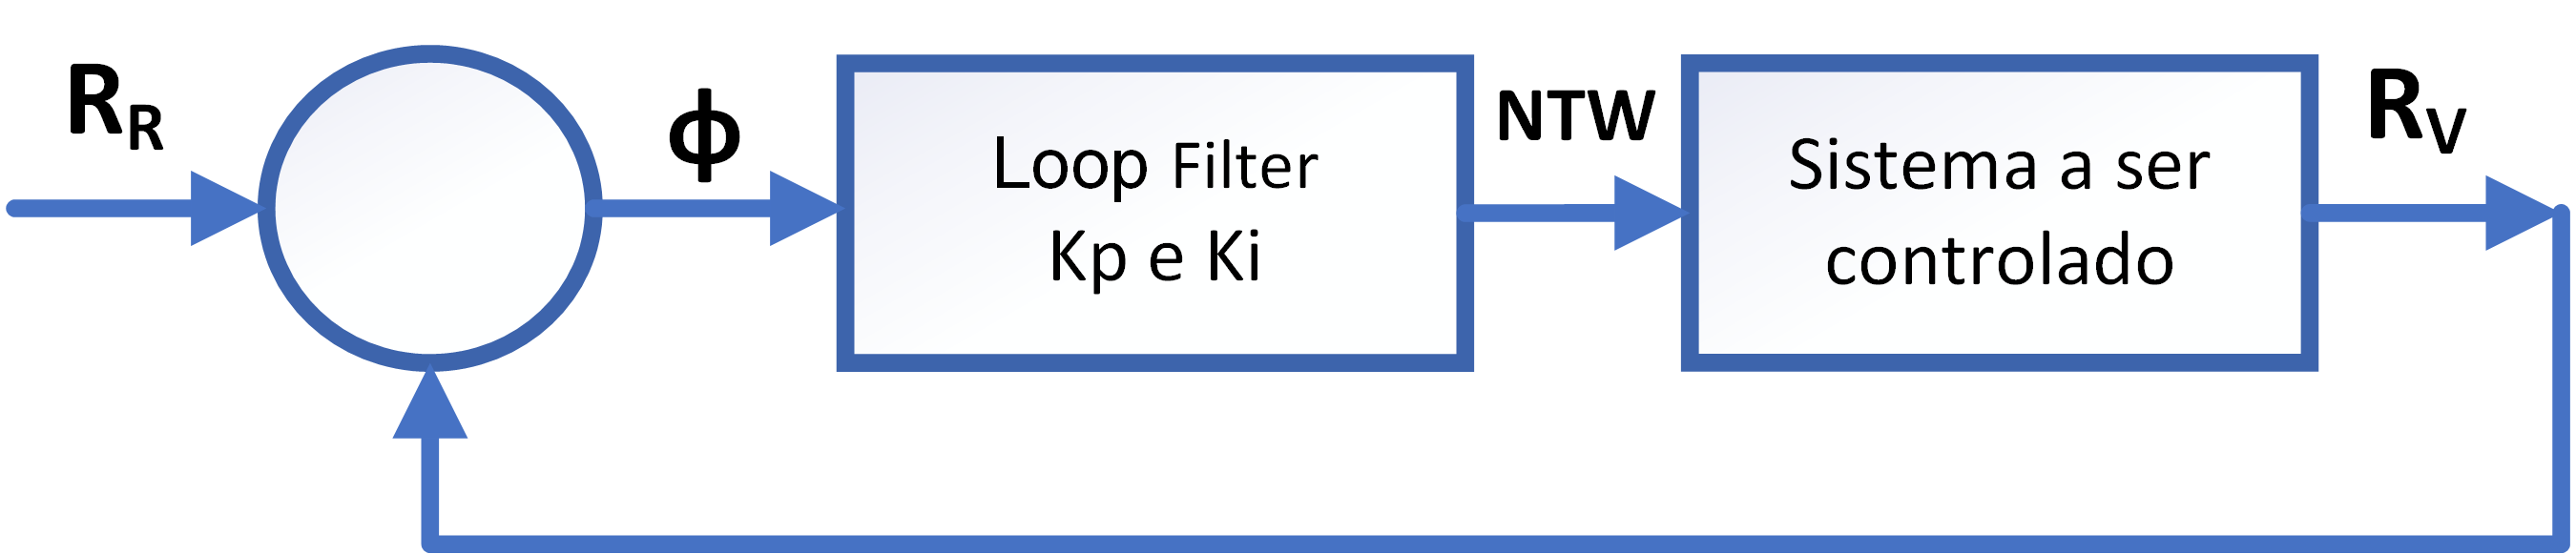
\includegraphics[scale=0.7]{img/loop_filter_PI.png}
	\label{fig:loop_filter_PI}}
	\hfil
	\subfloat[\textit{Loop Filter} no domínio Z]{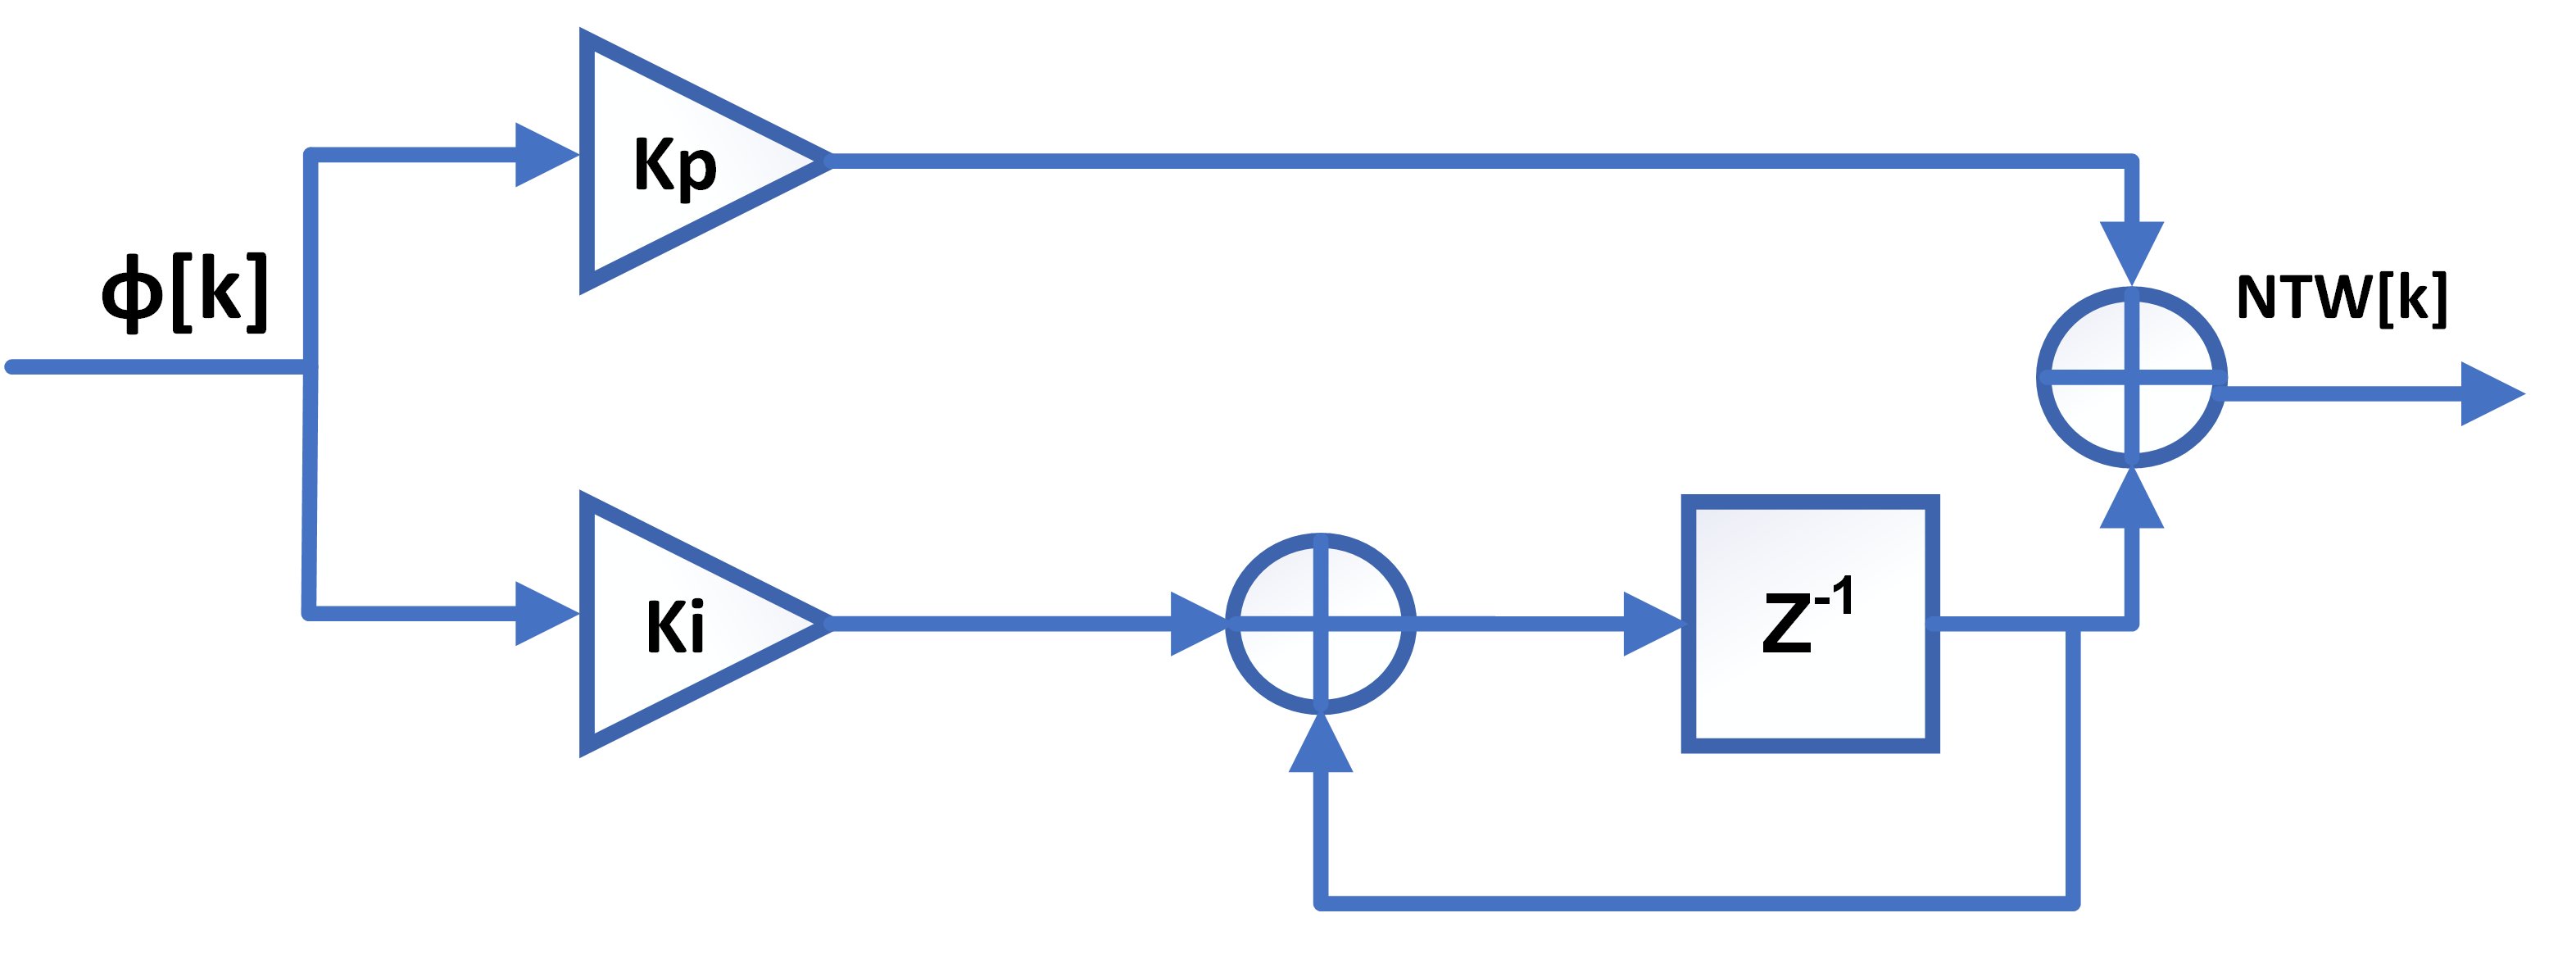
\includegraphics[scale=0.7]{img/loop_filter_typeII.png}
		\label{fig:loop_filter_typeII}}
	\end{center}
	\fonte{Adaptado de \citeonline{andersson2010modeling}.}
	\label{fig:loop_filter_structure}
\end{figure}

 O \textit{Loop Filter} mostrado na Figura \ref{fig:loop_filter_typeII} é classificado  como ADPLL Tipo II, pois incorpora  o ganho proporcional (P) e o integrador (I). Sua expressão de tempo discreto que descreve seu comportamento é mostrado em \ref{eq:ntw_type2}. Por outro lado, o ADPLL Tipo I é definido quando contém apenas o ganho proporcional,  reduzindo a expressão para uma simples multiplicação, como mostrado em \ref{eq:ntw_type1}.
 
 \begin{equation}
 	NTW[k]= K_p \cdot \phi [k] - K_p \cdot \phi [k -1] + K_I \cdot \phi [k-1] + NTW[k-1]
 	\label{eq:ntw_type2}
 \end{equation}
 
 \begin{equation}
 	NTW[k]= K_p \cdot \phi [k] 
 	\label{eq:ntw_type1}
 \end{equation}
 
 
 
 O \textit{Loop Filter} é dividido em três blocos, um para controlar cada um dos modos do DCO  permitindo a utilização independente do ADPLL Tipo I ou Tipo II em cada modo. Nos modos PVT e ACQ, o ADPLL Tipo I utilizado para reduzir o tempo de convergência do sistema, pois nesses modos o ajuste de frequência é mais grosseiro. No modo TRK, o ADPLL Tipo II é utilizado para obter a melhor precisão, onde o integrador é inserido para reduzir o erro e o valor do ganho proporcional é reduzido.
 
 Um filtro IIR passa-baixa \textit{Infinite Impulse  Response} pode ser conectado em cascata antes do \textit{Loop Filter} caso seja necessário  atenuar ruídos de fase e espúrios indesejados em altas frequências. É importante dimensioná-lo de forma que a frequência de corte seja maior que a do \textit{Loop Filter}, para não afetar seu desempenho.
 
 
Filtro IRR de ordem simples é incondicionalmente estável, porém possui uma pequena atenuação. Para obter maiores atenuações pode ser necessário filtro de ordem superior
mas isso pode torná-los facilmente instáveis. filtros de ordem simples em cascata podem ser utilizados, como mostrado na Figura \ref{fig:filter_IRR}. Essa configuração proporciona maior atenuação de ruídos indesejados sem comprometer a estabilidade do sistema.

\begin{figure}[h!]
	\caption{\textit{Loop Filter} com filtro IIR em cascata}
	\begin{center}
		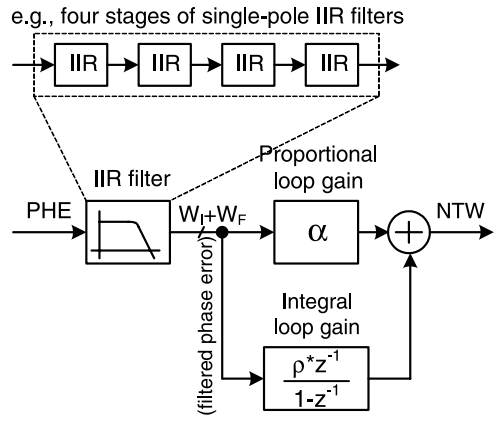
\includegraphics[scale=0.8]{img/filter_IRR.png}
	\end{center}
	\fonte{ \citeonline{StaszewskinDCO}.}
	\label{fig:filter_IRR}
\end{figure}

O Filtro IRR pode ser analisado no domínio do tempo discreto de acordo com a Figura \ref{fig:filter_IRR_time_domain}.

\begin{figure}[h!]
	\caption{Filtro IRR de polo simples}
	\begin{center}
		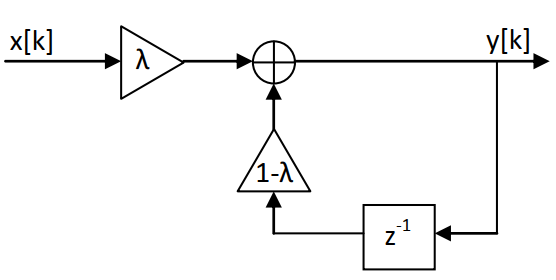
\includegraphics[scale=0.8]{img/filter_IRR_time_domain.png}
	\end{center}
	\fonte{ \citeonline{andersson2010modeling}.}
	\label{fig:filter_IRR_time_domain}
\end{figure}

A expressão no tempo discreto do IRR de polo simples é mostrada na equação \ref{eq:irr_simple_pole}, o que resulta na função de transferência no domínio Z conforme a equação \ref{eq:irr_tranfer_function}.

 \begin{equation}
	y[k]= (1 - \lambda) y[k-1] + \lambda x[k]
	\label{eq:irr_simple_pole}
\end{equation}

 \begin{equation}
	H_{IIR}(z)= \frac{z \lambda}{z -1 + \lambda}
	\label{eq:irr_tranfer_function}
\end{equation}


O termo $\lambda$ determina características importantes do filtro, como atenuação fora da banda de passagem e frequência de corte. Estes valores podem ser obtidos de acordo com a equação \ref{eq:iir_fbw}.


 \begin{equation}
	f_{BW_{IIR}}= \frac{\lambda}{2 \pi} f_{ref}
	\label{eq:iir_fbw}
\end{equation}

A função de transferência de um conjunto de filtros IRR de polo simples é obtida pelo produto de cada estágio como demonstrada na equação \ref{eq:filter_ir_prod}.

 \begin{equation}
	H_{IIR_{tot}}(z)= \prod 	H_{IIR_{simgle}}(z)
	\label{eq:filter_ir_prod}
\end{equation}

%%%%%%%%%%%%%%%%%%%%%%%%%%%%%%%%%%%%%%%%%%%%%%%%%%%%%%%%%%%%%%%%%%%%%%
\subsection{TDC}
%%%%%%%%%%%%%%%%%%%%%%%%%%%%%%%%%%%%%%%%%%%%%%%%%%%%%%%%%%%%%%%%%%%%%%

O TDC (Time to Digital Converter) utilizado no\textit{ Phase Detector} é responsável por medir com grande precisão a diferença de tempo entre a borda de clock de referência e a borda imediatamente anterior da saída do sintetizador. Esta diferença de tempo é a diferença de fase fracional entre os sinais na frequência. 

Existem diferentes topologias de circuitos para implementar um TDC, sendo algumas delas baseadas em cadeias de inversores, conhecidas como "\textit{delays}". Em tecnologias de processo CMOS atuais, é possível obter \textit{delays} com precisão de até $10 ps$ ou menos. \cite{ferreira2020review} apresenta diferentes topologias de circuito para implementação de um TDC baseado em cascata de inversores.

A medição de tempo é realizada pelo diferença de tempo $\Delta t_r$ medida em múltiplos inteiros de \textit{delays} simples $\Delta t_{res}$ em segundos conforme apresentado na Figura \ref{fig:tdc_chain_delayed}. O número de estágios do TDC é definido pelo número de inversores necessários para cobrir todo o período do \textit{clock} CKV. Dado que a resolução o TDC é limitada a $\Delta t_{res}$ somente múltiplos deste valor podem ser obtidos, desta forma, a medida é quantizada em $\Delta t_r\_Q$ conforme mostrada na Figura \ref{fig:tdc_quantization}.


% entre as bordas do sinal de referência e de saída, como mostrado na . Essa informação é fundamental para calcular o erro de fase $\phi$, necessário para sincronizar a saída do sintetizador com a frequência de referência.
%
%A resolução do TDC é definida pelo valor do atraso de um único inversor "\textit{delay}" utilizado, desta forma 
%
%Portanto, um erro de quantização $\Delta t_{r_Q}$ está associado à medida realizada como mostrado na Figura \ref{fig:tdc_erros_qtd}. O erro de quantização representa a menor diferença de tempo que o TDC pode medir com precisão. O

%Por exemplo, se o atraso de um inversor for de $10 ps$, o TDC só poderá medir diferenças de tempo múltiplas desse valor, como $10 ps$, $20 ps$, $30 ps$, e assim por diante. Qualquer diferença de tempo menor do que $10 ps$ será arredondada para o valor mais próximo múltiplo de $10 ps$, introduzindo o erro de quantização. Esse erro deve ser levado em consideração na análise do desempenho do sistema ADPLL perincipalmente na questão de ruido de fase.


%\begin{figure}[h!]
%	\caption{Diferença de tempo medida pelo número de inversores \textit{delays}}
%	\begin{center}
%		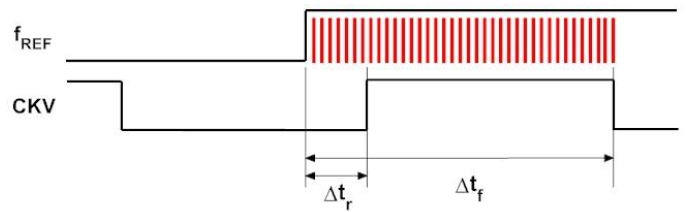
\includegraphics[scale=0.8]{img/tdc_tr_tf.png}
%	\end{center}
%	\fonte{ \citeonline{andersson2010modeling}.}
%	\label{fig:tdc_tr_tf}
%\end{figure}


\begin{figure}[h!]
	\caption{TDC }
	\begin{center}
		\subfloat[Impelemntação em Hardware]{	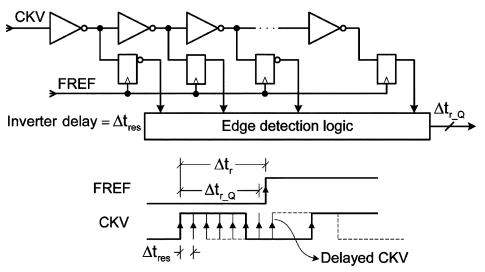
\includegraphics[scale=0.7]{img/tdc_chain_delayed.png}
			\label{fig:tdc_chain_delayed}}
		\hfil
		\subfloat[Modelo comportamental]{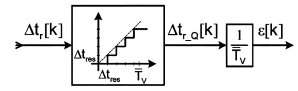
\includegraphics[scale=0.7]{img/tdc_quantization.png}
			\label{fig:tdc_quantization}}
	\end{center}
	\fonte{\citeonline{syllaios2008time}.}
	\label{fig:tdc_harware}
\end{figure}


A diferença de fase fracional que é a saída do TDC é obtida conforme a equação \ref{eq:tdc_error_quanti}, onde $\Delta t_r\_Q$ é normalizado em relação ao período de CKV.

%\begin{figure}[h!]
%	\caption{Quantização do TDC}
%	\begin{center}
%		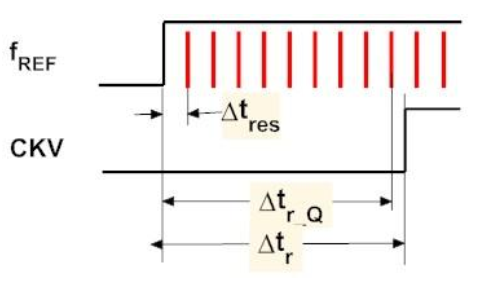
\includegraphics[scale=0.8]{img/tdc_erros_qtd.png}
%	\end{center}
%	\fonte{ \citeonline{andersson2010modeling}.}
%	\label{fig:tdc_erros_qtd}
%\end{figure}

 \begin{equation}
	\epsilon [k]= 1 - \frac{1}{\bar T_{CKV}} \cdot \Delta t_{res} \cdot \Bigg ( \frac{\Delta t_r [k]}{ \Delta t_{res}} \Bigg )  = 1 - \frac{\Delta t_r\_Q[k]}{\bar{T}_{CKV}}
	\label{eq:tdc_error_quanti}
\end{equation}

Onde $\bar T_{CKV}$ é obtido pela média de CKV em um determinado período de tempo conforme mostrado na equação \ref{eq:tdc_tckv_avg}.

 \begin{equation}
\bar T_{CKV}= \frac{1}{N_{avg}} \cdot \sum_{l=1}^{N_{avg}} ( t_{CKV}[l] - t_{CKV}[l-1])
	\label{eq:tdc_tckv_avg}
\end{equation}

%%%%%%%%%%%%%%%%%%%%%%%%%%%%%%%%%%%%%%%%%%%%%%%%%%%%%%%%%%%%%%%%%%%%%%
\section{Ruído de Fase}
%%%%%%%%%%%%%%%%%%%%%%%%%%%%%%%%%%%%%%%%%%%%%%%%%%%%%%%%%%%%%%%%%%%%%%

Em um oscilador ideal operando na frequência $\omega_c$ toda potência é concentrada em $\omega_c$, já em um oscilador prático a a potência se espalha perto de $\omega_c$ como mostrado na Figura \ref{fig:phase_noise_ideal_practical}, sendo este espalhamento chamado de ruido de fase. Nos transmissores o ruido de fase pode interferir em canais adjacentes, enquanto no receptor afeta a seletividade do mesmo.

O ruido de fase é quantizado considerando uma largura de banda de $1Hz$ distante a $\Delta \omega$ da frequência central $\omega_c$, sendo a unidade de medida dada em (dBc/Hz), onde "c" do "dBc" é convencionado como uma medida em relação a portadora (\textit{carrier}).

\begin{figure}[h!]
	\caption{Espectro de saída de um oscilador ideal e um oscilador prático}
	\begin{center}
			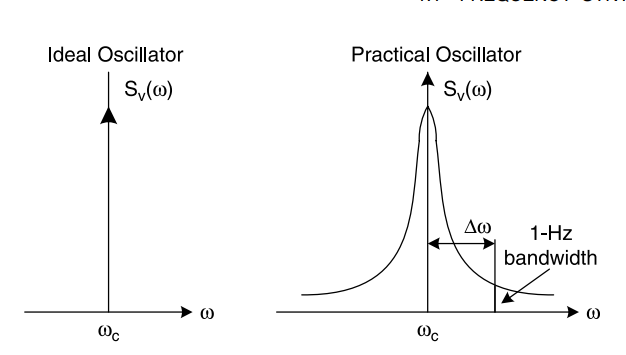
\includegraphics[scale=0.8]{img/phase_noise_ideal_practical.png}
		\end{center}
	\fonte{ \citeonline{staszewski2006all}.}
	\label{fig:phase_noise_ideal_practical}
\end{figure}

Ruido de fase pode ser analisado no domínio da frequência expressando a saída como $v(t) = A cos(\omega_c t + \phi)$, onde A é a amplitude, $\omega_c$ a frequência e $\phi$ é um deslocamento de fase. Tanto amplitude como $\phi$ podem sofrer variações, a amplitude é facilmente removida com um circuito limitador, porém a fase causa variações no período do sinal sendo o ruido de fase.


A Figura \ref{fig:phase_noise_spectrum} mostra o espetro \textit{single side}  tipico de ruido de fase um oscilador. O gráfico em escala logarítmica normalizado em dBc/Hz é exibido com um deslocamento $\Delta \omega$ da portadora $\omega_c$. 

\begin{figure}[h!]
	\caption{Espectro de ruido de fase de um oscilador}
	\begin{center}
		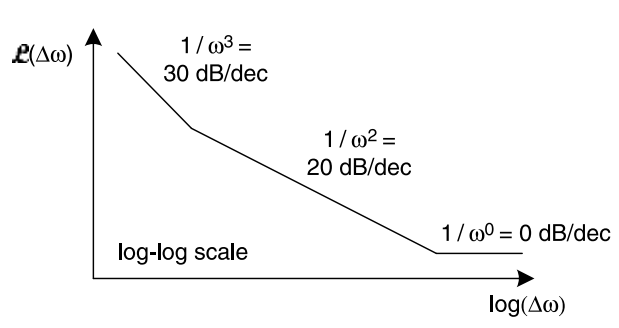
\includegraphics[scale=0.8]{img/phase_noise_spectrum.png}
	\end{center}
	\fonte{ \citeonline{staszewski2006all}.}
	\label{fig:phase_noise_spectrum}
\end{figure}

A região $\/\omega^2$ é conhecida como região de ruido térmico (\textit{thermal noise}) ou \textit{wander noise}, causado por ruido branco ou não correlacionado flutuações no período do oscilador. É o ruido dominante no DCO de acordo com \cite{staszewski2006all}.

A região plana $1/\omega ^0$ é definida como \textit{jitter noise} causando pequenas flutuações a cada período do oscilador.

A região $1/\omega ^3$ é resultado do \textit{up-converted} $1/f$ \textit{noise}, conhecido como ruido de \textit{flicker} que afeta todos dispositivos eletrônicos. Ele é dominante em baixas frequências sendo não tão presente no DCO que opera em altas frequências, mas que pode impactar no receptor gerando problemas de intermodulação.

No ADPLL os blocos mais críticos como geradores de ruido são o DCO, e o TDC. O DCO pela sua complexidade de utilização de bancos de capacitores e ruido térmico, e o TDC além do ruido térmico pelo erro de quantização causando variações de tempo. Esse ruido do TDC pode ser calculado conforme a equação \ref{eq:tdc_noise}.


 \begin{equation}
	\mathcal{L} = \frac{(2 \pi)^2}{12} \bigg (  \frac{\Delta t_{res}}{\bar{T}_{CKV}}\bigg)^2 \frac{1}{f_{ref}}
	\label{eq:tdc_noise}
\end{equation}

%%%%%%%%%%%%%%%%%%%%%%%%%%%%%%%%%%%%%%%%%%%%%%%%%%%%%%%%%%%%%%%%%%%%%%
%\section{Modelo no domínio S}
\section{Resposta em frequência do ADPLL}
%%%%%%%%%%%%%%%%%%%%%%%%%%%%%%%%%%%%%%%%%%%%%%%%%%%%%%%%%%%%%%%%%%%%%%

O estudo da resposta em frequência do ADPLL é necessária para analisar o comportamento do sistema, como estabilidade, tempo de acomodação (\textit{settling time}), e largura de banda do \textit{loop}. Para isto o sistema é modelado no domínio de frequência S verificando os polos e zeros do sistema. A Figura \ref{fig:adpll_type_II_s_domain} mostra o equivalente de um ADPLL Tipo II em análise no domínio S inserido fontes de ruido. 

\begin{figure}[h!]
	\caption{Modelo no dominio S de um ADPLL Tipo II com fontes de ruido incluídas}
	\begin{center}
		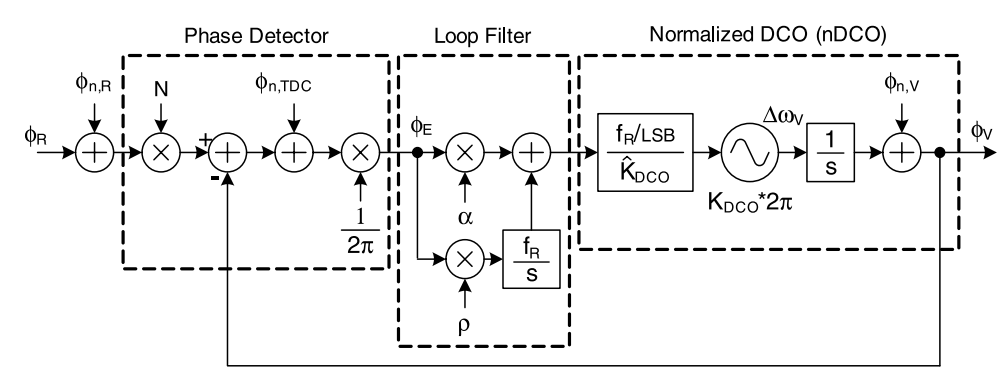
\includegraphics[scale=0.6]{img/adpll_type_II_s_domain.png}
	\end{center}
	\fonte{ \citeonline{staszewski2006all}.}
	\label{fig:adpll_type_II_s_domain}
\end{figure}

As siglas da figura representam:

\begin{itemize}
	\item $\phi_{R}$ = Fase de referência
	\item $N$ = FCW
	\item $\phi_{n,TDC}$ = Fonte de ruido do TDC
	\item $\alpha$ = $K_P$ ganho proporcional
	\item $\rho$ = $K_I$ ganho do integrador
	\item $\phi_{n,DCO}$ = Fonte de ruido do DCO
\end{itemize}

Assumindo que $K_{DCO}$ está corretamente estimado e desconsiderando as fontes de ruido, obtém-se a função de transferência de \textit{loop} aberto como mostra a equação \ref{eq:hol_s_adpll_tipe_II}.

	\begin{equation}
	H_{ol}(s) = \big( \alpha + \frac{\rho f_R}{s} \big) \frac{f_R}{s} = \frac{\rho f_R^2}{s} \cdot \frac{1 + s/(\rho f_R / \alpha)}{s}
	\label{eq:hol_s_adpll_tipe_II}
	\end{equation}
Disto obtêm-se dois polos na origem $\omega_p1 = \omega_p2 = 0$, e um zero complexo em $\omega_z = j(\rho f_R / \alpha) $

A função de transferência em \textit{loop} fechado para o sinal de referencia como estrada é mostrada na equação \ref{eq:hol_s_adpll_tipe_II}, ela comporta-se como um filtro passa-baixa com ganho dado pelo valor de N.

	\begin{equation}
	H_{REF}(s) = N\frac{ ( \alpha + \rho f_R/s)(f_R/s)}{1 + (\alpha + \rho f_R/s) (f_R/s)} =  N\frac{ \alpha f_R s + \rho f_R^2}{s^2 + \alpha f_R s + \rho f_R^2}
	\label{eq:hcl_s_adpll_tipe_II}
	\end{equation}

Fazendo a mesma análise considerando as fontes de ruido do TDC ( $\phi_{n,TDC}$) e do DCO ( $\phi_{n,DCO}$) obtém-se:

	\begin{equation}
	H_{TDC}(s) =\frac{ \alpha f_R s + \rho f_R^2}{s^2 + \alpha f_R s + \rho f_R^2}
	\label{eq:tdc_s_adpll_tipe_II}
	\end{equation}
	
	\begin{equation}
	H_{DCO}(s) = \frac{s^2}{s^2 + \alpha f_R s + \rho f_R^2}
	\label{eq:dco_s_adpll_tipe_II}
	\end{equation}

Nota-se nque todas as funções de transferência de \textit{loop} fechado contém o mesmo denominador, sendo igual a $ 1 + H_{ol}(s)$, assim pode-se fazer uma simplificação como mostrado na equação \ref{eq:hcl_simplification}.


	\begin{equation}
	H_{REF}(s) =  \frac{1}{1 + H_{ol}(s)} \hspace{1cm}
	H_{TDC}(s) =  \frac{ H_{ol}(s)}{1 + H_{ol}(s)} \hspace{1cm}
	H_{DCO}(s) =  \frac{N \cdot H_{ol}(s)}{1 + H_{ol}(s)} \hspace{1cm}
	\label{eq:hcl_simplification}
\end{equation}

A função de \textit{loop} fechado pode ser comparada a função de transferência tradicional de um sistema de duplo polo mostrada na equação  

	\begin{equation}
	H_{REF}(s) =   N\frac{ 2 \zeta \omega_n s +  \omega_n^2}{s^2 + \zeta  \omega_n s + \ \omega_n^2}
	\label{eq:classical_two_pole}
	\end{equation}

onde $\zeta$ é o fator de amortecimento, e $\omega_n$ a frequência natural, tendo um zero em $\omega_z = - \omega_n / 2 \zeta$. Assim:


	\begin{equation}
	\omega_n = \sqrt{\rho} f_r
	\label{eq:omena_n}
	\end{equation}	
	
	\begin{equation}
		\zeta =   \frac{\alpha f_r}{2 \zeta \omega_n} = \frac{1}{2} \big (  \frac{\alpha}{\sqrt{\rho}}\big )
		\label{eq:qsi}
	\end{equation}

A transformada de Laplace utilizada no domínio S é para sistemas de tempo continuo, enquanto para sistemas discretos como é o caso do ADPLL é correto utilizar o domínio discreto Z. Domínio S facilita na análise do sistema facilmente podendo ser encontrado os polos e zeros e verificar parâmetros importantes em um sistema, porém, o tempo discreto pode ser aproximado ao domínio S se a frequência de amostragem for muito maior que a de interesse. 

O operador $Z$ é definido como $Z^{j\theta}$, sendo $\theta = \omega t_0$, $\omega = 2 \pi f$ a frequência angular e $t_0$ o período de amostragem, no caso $t_0 = 1/f_R$. Assim o operador Z é definido conforme a equação \ref{eq:z_operator}.


	\begin{equation}
	Z^{j\theta} = Z^{j\omega /f_R}
	\label{eq:z_operator}
	\end{equation}


Sendo $\omega << f_R$ e aplicando algumas propriedades trigonométricas chega-se que a conversão de S para Z é dada pela equação \ref{eq:s_to_z}.

	\begin{equation}
	s = f_R(z - 1)
	\label{eq:s_to_z}
	\end{equation}


Aplicando a conversão nas equações \ref{eq:hol_s_adpll_tipe_II} e \ref{eq:hcl_s_adpll_tipe_II} obtêm-se as equações mostradas em \ref{eq:hol_z_adpll_tipe_II} e \ref{eq:hcl_z_adpll_tipe_II} respectivamente.

	\begin{equation}
	H_{ol}(z) = \frac{ \alpha (z - 1) + \rho}{ (z - 1)^2}
	\label{eq:hol_z_adpll_tipe_II}
	\end{equation}

	\begin{equation}
	H_{cl}(z) = N \frac{ \alpha (z - 1) + \rho}{ (z - 1)^2 + \alpha (z - 1) + \rho}
	\label{eq:hcl_z_adpll_tipe_II}
	\end{equation}


Quando utilizado filtro IRR como visto na seção \ref{sec:loop_filter} no \textit{lopp filter}, as funções de transferência do sistema devem considerar seus impactos.

Da equação \ref{eq:irr_tranfer_function} de um filtro IRR de polo simples a função de transferência no domínio S é mostrada na equação \ref{eq:irr_s_domain}.

	\begin{equation}
	[H_{iir}(s) = \frac{ 1 + s/f_R}{ 1 + s/\lambda f_R}
	\label{eq:irr_s_domain}
	\end{equation}
	
Assim a função de transferência de \textit{loop} aberto é alterada para:


\begin{equation}
	H_{ol}(s) = \frac{\rho f_R^2}{s} \cdot \frac{1 + s/(\rho f_R / \alpha)}{s} \cdot \frac{f_R}{s} \frac{ 1 + s/f_R}{ 1 + s/\lambda f_R}
	\label{eq:hol_irr_simgle}
\end{equation}


Sendo o filtro IRR com mais de um estágio e valores de $\lambda$ diferentes em cada $H_{ol}(s)$ resume-se a:

\begin{equation}
H_{ol}(s) = \frac{\rho f_R^2}{s} \cdot \frac{1 + s/(\rho f_R / \alpha)}{s} \cdot \prod_{i=1}^{n} \frac{f_R}{s} \frac{ 1 + s/f_R}{ 1 + s/\lambda_i f_R}
	\label{eq:hol_irr_cascade}
\end{equation}


%%%%%%%%%%%%%%%%%%%%%%%%%%%%%%%%%%%%%%%%%%%%%%%%%%%%%%%%%%%%%%%%%%%%%%
\section{Trabalhos correlatos}
%%%%%%%%%%%%%%%%%%%%%%%%%%%%%%%%%%%%%%%%%%%%%%%%%%%%%%%%%%%%%%%%%%%%%%
Nesta seção, serão apresentados alguns trabalhos relacionados ao tema deste estudo, que envolve o desenvolvimento e simulação de um ADPLL em tecnologia CMOS. Esses trabalhos servirão como base e referência para o desenvolvimento neste trabalho.

O trabalho de Ioannis L. Syllaios em \cite{syllaios2008time} fornece um modelo de domínio do tempo para um ADPLL com aplicação em RF. Através deste modelo, o autor realiza uma análise detalhada do comportamento do circuito, abordando aspectos de projeto, desempenho e estabilidade. A simulação feita utilizando Matlab, e análise propostas nesse trabalho serão utilizadas como referência para a simulação do ADPLL desenvolvido neste estudo.

Em \cite{staszewski2006all} Robert Bogdan Staszewski  apresenta um sintetizador de frequência totalmente digital implementado em tecnologia CMOS. O autor apresenta detalhadamente toda a estrutura de um ADPLL, e todas suas peculiaridades, discute=indo os desafios de implementação do ADPLL em tecnologias avançadas e destaca as vantagens do uso de uma abordagem totalmente digital em relação às soluções analógicas tradicionais. Essas informações são de grande importância para o dimensionamento do ADPLL principalmente quanto a analise de frequência e ruido de fase.


O trabalho de Andersson Fredrik em \cite{andersson2010modeling} aborda a modelagem e caracterização de um ADPLL totalmente digital para uma aplicação WCDMA. A simulação feita em Matlab possibilita a análise do desempenho em diferentes condições de operação. A modelagem e análise pelo autor elaborada auxiliam no desenvolvimento deste trabalho.

%%%%%%%%%%%%%%%%%%%%%%%%%%%%%%%%%%%%%%%%%%%%%%%%%%%%%%%%%%%%%%%%%%%%%%
\section{Considerações Finais}
%%%%%%%%%%%%%%%%%%%%%%%%%%%%%%%%%%%%%%%%%%%%%%%%%%%%%%%%%%%%%%%%%%%%%%

A Revisão Bibliográfica apresentou alguns conceitos e descrição comportamental do ADPLL em blocos. Tais informações são importantes para que se possa ser implementado na Metodologia.
%%%%%%%%%%%%%%%%%%%%%%%%%%%%%%%%%%%%%%%%%%%%%%%%%%%%%%%%%%%%%%%%%%%%%%

